\documentclass[11pt]{report} 
%
\usepackage{projectreport}
\newcommand{\projecttitle}{CFD Simulation and Investigation of Slurry Flows in Pipelines}
\newcommand{\name}{Marwane ElKarii}
\newcommand{\course}{}
\newcommand{\submissiondate}{Octorber 2021}

\usepackage{concmath}
\usepackage[OT1]{fontenc}
\usepackage{subcaption}


%%%%%%%%%%%%%%%%%%%%%%%%%%%%%%%%%%%%%%%%%%%%%%%%%%%%%%%%%%%%%%%%%%%%%%%%%%%%%%%%%%%%%%%%%%%%%%%%%%%%
\begin{document}
%%%%%%%%%%%%%%%%%%%%%%%%%%%%%%%%%%%%%%%%%%%%%%%%%%%%%%%%%%%%%%%%%%%%%%%%%%%%%%%%%%%%%%%%%%%%%%%%%%%%
\maketitle
\tableofcontents
\renewcommand{\thepage}{\arabic{page}}
%%%%%%%%%%%%%%%%%%%%%%%%%%%%%%%%%%%%%%%%%%%%%%%%%%%%%%%%%%%%%%%%%%%%%%%%%%%%%%%%%%%%%%%%%%%%%%%%%%%%
\chapter{Introduction}
\label{chap:intro}
%%%%%%%%%%%%%%%%%%%%%%%%%%%%%%%%%%%%%%%%%%%%%%%%%%%%%%%%%%%%%%%%%%%%%%%%%%%%%%%%%%%%%%%%%%%%%%%%%%%%
Pipeline transport of solid-liquid sludge is an essential operation in many areas, such as mining and chemical processing.
%
This comes down to the fact that pipelines are more efficient and environmentally friendly than railway transportation.
%
Yet, the transported fluid may be highly viscous and have complex rheology.
%
Moreover, the flow within the pipe is  generally highly turbulent and complex (\citet{Lahiri-2010}) and problems like pipe plugging, and solid sedimentation could occur.
%
Therefore, to ensure a continuous and optimal flow, different parameters should be controlled.
%
In particular, the distribution of solids and the pressure drop within the pipeline represent a serious concerns to engineers, since their determination involves considerable technical difficulties.
%
Thus, having means to predict the physics of the slurry flow is essential for the control of the pipeline process.
%
The rapid increase in computational power has made it possible to widely distribute different tools and techniques, capable of modeling complex flows in real-dimensional geometries.
%
This paved for a better handling of such flows by complementing empirical methods with digital simulations.
%
Therefore, Computational Fluid Dynamics (CFD) has appeared as an effective tool to model and predict unknown or particular slurry flow scenarios (\citet{Bi-2002}), and it can provide a series of monitoring information, which is difficult to achieve by experience alone.
%
The advantages of CFD can be categorized as
%
\begin{itemize}
\item It provides a detailed understanding of flow distribution, mass and heat transfer, particulate separation, etc.
%
Consequently, all these will lead to a much better and deeper understanding of what is happening in a particular process or system.
%
\item It is able to reduce scale-up problems because the models are based on fundamental physics and are scale independent.
%
\item It is particularly useful in simulating conditions where it is not possible to take detailed measurements.
\end{itemize}
%%%%%%%%%%%%%%%%%%%
\section{CFD approaches for multiphase flows}
Generally, the CFD approaches for the simulation of slurry flows can be classified into:
\begin{itemize}
\item Eulerian-Lagrangian approaches (\cite{crowe-2011}), where the liquid phase is modeled as a continuum and solved in an Eulerian cell-based framework, whereas the behavior of the solid phase is obtained by the Discrete Particle Method (DPM), in which the individual trajectories of computational particles are calculated in a Lagrangian fashion.
%
\item Eulerian-Eulerian approaches (\cite{crowe-2011}), where  both phases are modeled as interpenetrating continua, and two sets of conservation equations are solved jointly in the Eulerian framework.
%
The coupling between the two phases depends on the amount of solids in the flow, and it ranges from one-way coupling for dilute slurries (\textit{i.e.}, the particles do not affect the liquid flow field) to four-way coupling for dense slurries (where the particle-particle and particle-fluid interactions are important as well).
%
This approach characterizes the majority of the earlier CFD investigations of slurry pipe flows which provides a good compromise between accuracy and computational cost.
%
Yet three models are possible within this approach.
\end{itemize}
%
Table \ref{tab:eul-eul-comp} shows a comparison of the latter models.
%
\begin{table}[ht!]
\caption{Comparison between Euler-Euler models}
\begin{tabular}{p{5.2cm}|p{5.2cm}|p{5.2cm}}
\hline 
VOF & 
Mixture Model & 
Multi-phase Eulerian Model 
\\\hline
Modelling non-miscible fluid &
Model used if there is a wide distribution of dispersed phases &
Interphase laws available. 
\\ \hline 
A single set of motion equations & 
Interphase laws not available & 
More precise. 
\\ \hline 
Examples: free surface flow (\cite{Jing-2016})), large bubbles in a liquid (\cite{Al-Yaari-2011})), stratified flow (\cite{Akhtar-2007})) & 
Examples: particle-laden flow* with low load (\cite{J-2007}), bubble flow, sludge flow (\cite{Liangyon-2009})  & 
Examples: sludge flow (\cite{Ofei-2016}), sedimentation ((\cite{gopaliya-2016}), fluidized beds (\cite{Ofei-2014})).\\
\hline
\end{tabular}
\label{tab:eul-eul-comp}
\end{table}
\footnote{Particle-laden flow = Particle charge flows refer to a two-phase flow in which one of the phases is continuously connected and the other phase consists of small immiscible particles and typically diluted.}
%%%%%%%%%%%%%%%%%%%%%%%%%%%%%%%%%%%%%%%%%%%%%%%%%%%%%%%%%%%%%%%%%%%%%%%%%%%%%%%%%%%%%%%%%%%%%%%%%%%%
\section{Problem Description}
%%%%%%%%%%%%%%%%%%%%%%%%%%%%%%%%%%%%%%%%%%%%%%%%%%%%%%%%%%%%%%%%%%%%%%%%%%%%%%%%%%%%%%%%%%%%%%%%%%%%
This work concerns the transport of phosphate ores in the context of an industry 4.0. The process begins with the extraction of ore that is transported as pulp (Water $+$ Phosphate) in a pipe (pipeline), from the mine to the industrial units for processing (cf. Fig.~\ref{fig:process-phosphate}). 
\begin{figure}[ht!]
\begin{center}
%\include{diag}
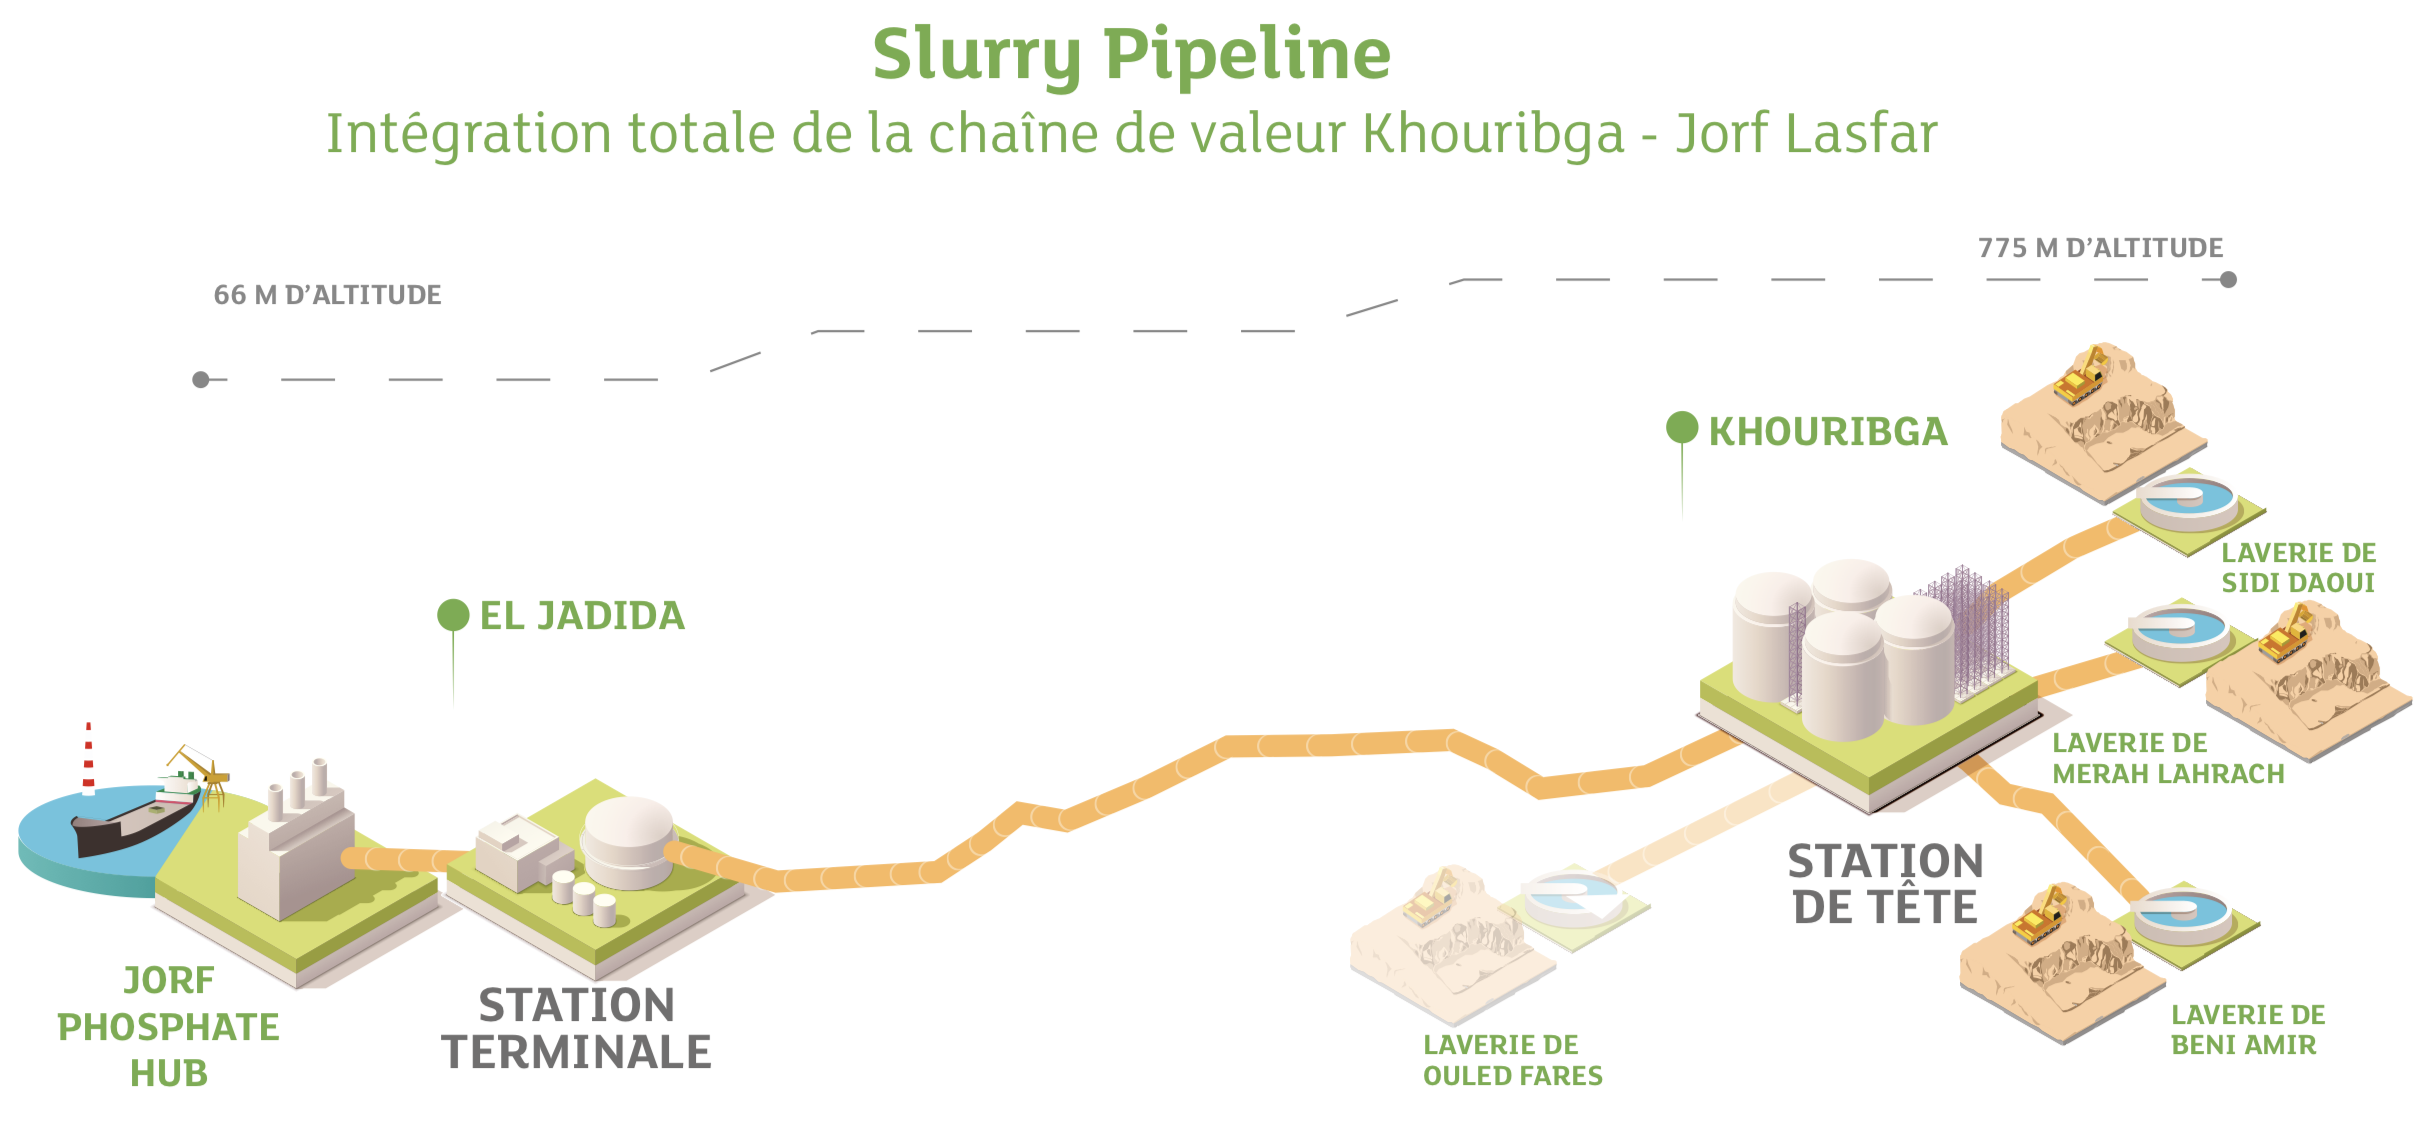
\includegraphics[width=12cm]{figs/pipe.png}
\caption{Transport process of phosphate slurry }
\label{fig:process-phosphate}
\end{center}
\end{figure} 
%
This pulp is characterized by a solid volume concentration that goes up  to 40 $\%$, it contains rigid solid particles of random shapes having an equivalent spherical diameter ranging from $44~\mathrm{\mu m}$ to $400~\mathrm{\mu m}$.
%
The ore particles are characterized by an average total porosity of 20 $\%$ by volume, then an effective density of $2600~\mathrm{kg/m^3}$ when the pores are filled with water.
%
The operation of the phosphate slurry pipe is controlled by a series of pressure and choke stations.
%
The pipeline receives the phosphate ore, of different qualities, from four different washing stations, which gives it variable flow properties (viscosity, density, speed, pressure...).
%
The phosphate pulp is transported in batches, separated by batches of water to control the quality and flow of the pulp (cf. Fig.~\ref{fig:phosphate-flow}). 
%
\begin{figure}[ht!]
\begin{center}
%\include{diag}
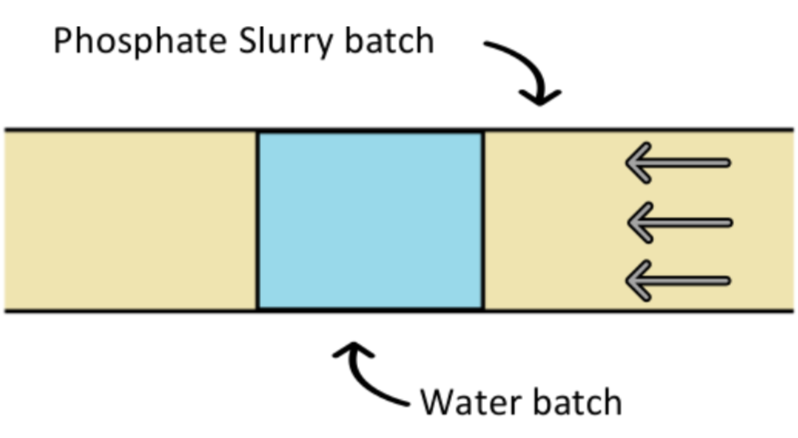
\includegraphics[width=8cm]{figs/batch.png}
\caption{Phosphate slurry flow}
\label{fig:phosphate-flow}
\end{center}
\end{figure} 

The main challenge of the work to be carried out in the context of this thesis is is to set the basis for an intelligent control for the transport process, based on computational fluid dynamics (CFD) simulation models.
%
This system will ensure optimal operation of the process, predict the evolution of certain critical parameters and contribute to operational decision-making.
%
From an application point of view, among the industrial stakes of the project of this thesis:
%
\begin{itemize}
\item Increase productivity (volume sent by the pipe);
\item Secure the pipe by mastering the characteristics of the pulp;
\item Predict solid concentration profiles and pressure losses in the pipeline;
\item Optimize pipe operation according to pulp quality;
\item Optimize energy consumption, etc;
\end{itemize}
%%%%%%%%%%%%%%%%%%%%%%%%%%%%%%%%%%%%%%%%%%%%%%%%%%%%%%%%%%%%%%%%%%%%%%%%%%%%%%%%%%%%%%%%%%%%%%%%%%%%
\chapter{Literature Review : slurry pipes modeling and simulation}
%%%%%%%%%%%%%%%%%%%%%%%%%%%%%%%%%%%%%%%%%%%%%%%%%%%%%%%%%%%%%%%%%%%%%%%%%%%%%%%%%%%%%%%%%%%%%%%%%%%%
%
A summary of the most relevant numerical studies on slurry flows in horizontal pipes published so far are reported, alongside with the adopted modelling approach.
%
Beginning with Eulerian-Lagrangian approach, this latter was employed for this kind of applications for sand-water slurry by \citet{Capecelatro-2013}, where the Large Eddy Simulation (LES) method \citet{versteeg2007introduction} has been used to simulate the turbulent flow of the liquid phase, while the solid phase was treated by DPM.
%
\citet{AROLLA20151} used the same numerical setup to characterize a sand-water flow pattern for increasing values of liquid superficial velocity.
%
Always in the Eulerian-Lagrangian approach but this time it was employed with different characteristics such as transportation of coarse NaCl particles in brine by \citet{Uzi-2017}, where the liquid phase is handled by a computationally cheaper Reynolds-Average Navier-Stokes (RANS) technique, to examine the effects of the operating conditions on the flow.
%
Concerning the mixture model, \citet{J-2003} performed CFD simulations for sand-water slurry flows through horizontal pipes, where a simplified 3D algebraic slip mixture (ASM) model is introduced along with RNG k–$\epsilon$ turbulent model to obtain the precise numerical solution in fully developed turbulent flow.
%
They compared CFD results of mean pressure gradients with experimental results, and found a big discrepancy between them takes place when the mean velocities of slurry flows are lower than corresponding critical deposition velocities.
%
\citet{C.X-2008} numerically investigated sand–water slurry flows in the entrance region of horizontal pipe, again using ASM model, and have focused mainly on illustrating and comparing the developing processes of various flow parameters.
%
\citet{Silva-2016} performed simulations for Saline Water-Glass beads slurry using Mixture Model coupled with a High Reynolds k–$\epsilon$ turbulence model, results were validated with data attained with an Electrical tomography apparatus.
%
The model produced accurate representations for the highest flow rates, while showing some deviations for the lower flow rate.
%
However, the majority of the earlier CFD investigations of slurry pipe flows were performed using the Two Fluid Model.
%
In most TFMs, constitutive equations for the solid phase derived from the Kinetic Theory of Granular Flow (KTGF) were employed.
%
The most relevant numerical studies on slurry flows in horizontal pipes published so far, the study of \citet{herna2008cfd} for sand-water slurry, where homogeneous and heterogeneous flow regimes without bed were considered along with predictions of pressure gradients at the fully developed zone.
%
\citet{Ekambara-2009} investigated the effect of in situ solids volume concentration, particle size, mixture velocity, and pipe diameter, on local time-averaged solids concentration profiles, particle and liquid velocity profiles, and frictional pressure loss.
%
Excellent agreement between the predicted and the experimental was obtained.
%
\citet{Liangyon-2009} used the same numerical configuration to simulate flow of coal-water slurries (CWS) in a horizontal pipeline, with bimodal distribution for coal particles.
%
They found out that the simulation results of the binary solid phase model is closer to experimental data, as compared to the results of the single solid phase model.
%
\citet{bossio2009eulerian} focused on modeling of non-Newtonian Laterite-Sand slurry where the mean pressure gradients were compared with experimental data.
%
\citet{antaya2012modelling}  performed simulations for concentrated mixtures of sand-water slurry with mono-sized and bimodal particle sizes.
%
Shear stress model (SST) was tested in addition to the k–$\epsilon$ model to treat the turbulence of the continuous  phase. Success has been achieved in the use of k–$\epsilon$ model,  with the SST model being superior, especially in the near-wall region.
%
However \citet{D.R-2012}, tried both  Mixture and  two-phase model to simulate mono-dispersed fine particles at high concentration of glass beads mixed with water.
%
They proved again the failure of the Mixture Model predictions at high velocities and high solid concentrations compared to TFM.
%
\cite{Y.Y-2012} worked on an unusual type of slurry flows which is Slush nitrogen flow using the 2D Eulerian – Eulerian multiphase approach.
%
The per-phase k–$\epsilon$ turbulence model is used in the study to model the turbulent two-phase flow.
%
The effects of the flow velocity and the mean solid volume fraction on the flow characteristics of slush nitrogen are investigated numerically in this study.
%
The same team in very next year \citet{Jiang-2013} investigated the same slush and nitrogen flow. Based on the experimental and numerical results they distinguished three flow patterns, which for each one they had studied the variation of pressure drop.
%
They obtained the general correlation of the friction factor with the slush Reynolds number of slush nitrogen with various solid volume fractions.
%
\citet{Wang-2013} applied the two fluid model to describe an ice slurry flow without considering ice melting.
%
After validation of the model with experimental data, it was used to investigate the distributions of ice slurry flow, ice particle concentration and pressure drop in horizontal, vertical and 90 elbow pipes respectively.
%
They found that for pressure drop, the numerical model is found being able to provide results in good agreement with the experimental data where the relative errors are limited to 20$\%$.
%
\citet{Messa-2013} developed a new two-fluid model for the simulation of Sand and Glass beads Water slurry.
%
Contrary to previous works with TFM models, they did not integrate the kinetic theory of granular flows to determine solid viscosity.
%
They studied the effect of the wall boundary condition for the solid phase on the pressure gradient, where they found that the best match between measurements and computations is obtained when the equilibrium logarithmic law of Launder and Spalding for smooth walls is applied to the solid phase.
%
Then, \citet{Messa-2014} used the new TFM model to  simulate a fully-suspended Sand-Water slurry flow in horizontal pipes and bends.
%
They claimed that the model is robust and numerically stable, and requires relatively short computer time to provide a converged steady-state solution.
%
The novelty of the proposed model and its better performance compared to similar ones reside in the method of accounting for some key physical mechanisms governing these flows, namely turbulent dispersion, interphase friction, and viscous and mechanical contributions to friction.
%
\citet{Messa-2015} further modified \citet{Messa-2014} model by incorporating a new wall boundary condition for the solid phase, a more general correlation for the viscosity of the slurry, accounting for particle shape along with a different solution algorithm. These changes resulted in low computational effort with improved performance.
%
They verified the modified model by comparing its outcomes with experimental results for sand-water slurries available in the literature. returning to the TFM combined with KTGF, \citet{Gopaliya-2014} studied the effects of grain size on various Sand-Water slurry flow parameters.
%
They found that at the same  volumetric concentration, pressure drop increases with increase in grain size.
%
\citet{Hashemi-2016} performed experiments in a 265 mm diameter pipe loop with sand-in-water slurries, then selected experimental conditions were  numerically simulated using a commercial CFD package, ANSYS CFX.
%
They noticed that the agreement between the numerical results and the experimental data is  concentration dependent, with relatively closer agreement at lower concentrations. 
%
\citet{kumar2019experimental} presented experimental data of iron-ore slurry flow cases through 105 mm pipe, the obtained results are validated using TFM-KTGF model. 
%
Results reflect good resemblance between measured and predicted pressure drops, solid concentrations and velocity profiles.
%
\citet{singh2020computational} investigated the flow characteristics of coal water slurry having high solid concentrations in slurry pipeline. 
%
They have noticed that the coal-water slurry shows Newtonian behaviour at 30$\%$ solid concentration (by-weight) and beyond this it depicts non Newtonian pseudo plastic behavior.
%
In this study also  SST k-$\omega$ turbulence model was found a better predictor over other models namely Standard k-$\epsilon$, RNG k-$\epsilon$, Realizable k-$\epsilon$ and Standard k-$\omega$ models. 
%
A year after \citet{Li-2018a} developed a useful three-dimensional multiphase hydrodynamic model based on the kinetic theory of granular flow, 
%
for simulating multi-sized glass beads-water slurry transport through pipelines, to investigate the distributions of solid concentration, flow velocity, granular pressure, and wall shear stress. 
%
The simulation results of different-sized particle behaviors in multi-sized slurry has significant reference value. 
%
\citet{Li-2018b} also in the same year studied the effect of interaction of particles with different sizes on particle kinetics in multi-sized slurry, 
%
first they concluded that the increase of speed of resistance  in a graded slurry is more gradual than in a single-sized slurry with the same conditions as the solid concentration increases, 
%
then they found that the wall shear stress of coarse particles is significantly reduced by the existence of fine particles with increasing flow rate and solid concentration, 
%
and finally they affirmed that the existence of fine particles significantly reduces the collision intensity of coarse particles and velocity fluctuations in the multi-sized slurry. 
%


%%%%%%%%%%%%%
\subsubsection{Summary on models classification}
Following the literature review presented above, our CFD approach will be based on the Eulerian model (Two Fluid Model) as it is the most complete model and the most used one to deal with suspensions transport issues, 
%
and is confirmed to be the most accurate and  gives generally good results.
%
While mixture model fails to predict pressure drops correctly and the amount of error increases rapidly with the slurry concentration  (\citet{D.R-2012}).  
%
The main conclusions from the literature review are summed in table 2. 
%
The description of the TFM model is given in section \ref{Model}. 
%
The dynamics of the solid phase is modeled by the KTGF to consider both particle collisions and frictions. 
%
Also, based on the previously cited works, the turbulence of the continuous phase is treated by the k-$\epsilon$ based models, that generally shows reasonable robustness, and give reasonable accuracy for a wide range of applications. 
%
Yet, even though success is usually achieved using models based on the k-epsilon, it should be made clear that they may not perform well in the region near the wall (\citet{antaya2012modelling}). 
%
Therefore, a near-wall treatment model is presented in section \ref{NWT}, to address the weak performance of the choosed turbulence models in this area of the pipe.
%
\begin{table}[ht!]
\caption{Summary on models classification }
\begin{tabular}{p{10cm}}
\centering
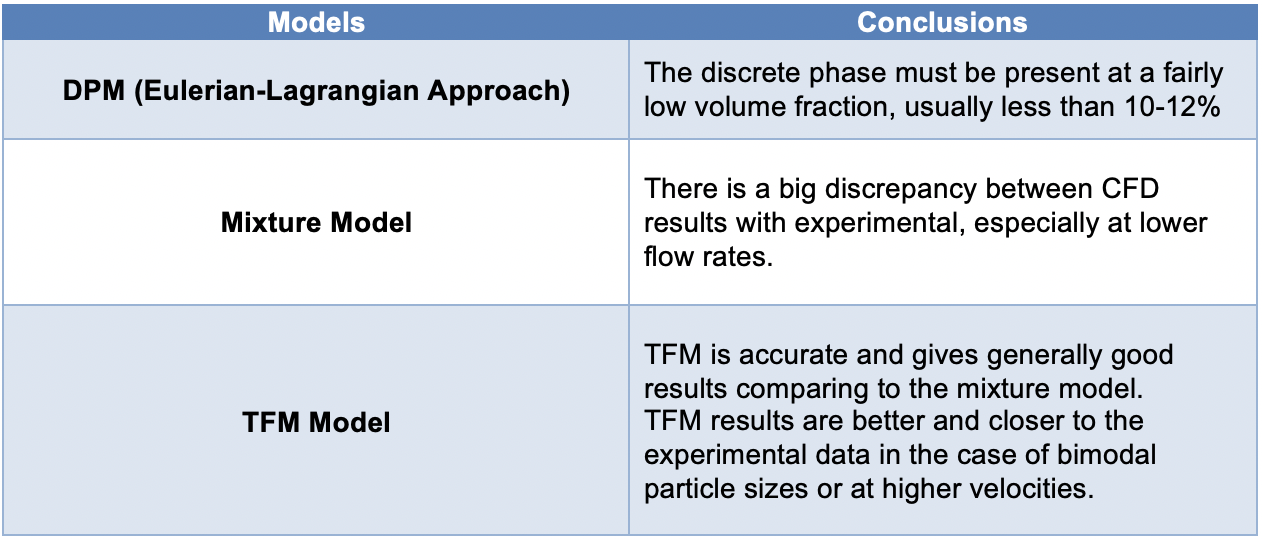
\includegraphics[trim=0cm 0cm 0cm 0cm,clip,scale= 0.69]{figs/class.png}
\end{tabular}
\end{table}

%%%%%%%%%%%%


%%%%%%
% a relire.... 
In fact,  modern modeling strategies, for industrial processes, integrates usually 3D simulation techniques using computational fluid dynamics (CFD) and/or discrete element methods (DEM). 
%
These 3D models are then integrated as surrogate models that can be used in operations simulation and monitoring tools (Decision Support Systems). 
%
Classically, response surface methodologies (RSM) are applied to build a polynomial surrogate model (\citet{Rabhi}), but also in recent works machine leaning techniques such as artificial neural networks (ANN) can be used (\citet{Seong}). 
%
The current modeling approach consists of  constructing 3D models for different type of pipe elements (horizontal, inclined, bended pipes), and then use them to construct surrogates that models the pressure drop within each element. 
%
Such models can then be used in dynamical models for monitoring slurry pipe systems and to conduct sizing studies to cover variations in the operation conditions like inlet pressure and inlet flow rate. 
%
This approach will first be applied to a single fluid flow to validate the approach of constructing a surrogate pressure drop model through 3D numerical simulation, 
%
and then to slurry flows with solid volume fraction corresponding to the applications that are aimed to cover.

A parametric analysis is conducted to investigate the impact of the variation in the particle size, solids concentration, and inlet velocity, 
%
on the solid concentration profile, the solid velocity profile and finally their effect on the variation in the pressure drop along the pipe. 
%
This analysis allows us to validates our simulations for turbulent slurry flows versus experimental data. 
%
The data used in this work is regarding a horizontal pipe case for Water-Sand slurry flow: transported solid volume fraction between 19  $\%$ and 45 $\%$; velocities between 1 m/s and 8.0 m/s; and particles sizes of 90 $\mu_m$ and 270 $\mu_m$. 





%The rest of this paper is structured in three sections. Section \ref{Theory} presents the adopted 3D, two-fluid, turbulent model for our simulations. Then in section \ref{results},  a validation of the approach on a single phase pipe flow is realized in (subsection \ref{single flow}). Then, and for the case of slurry flows, subsection \ref{Two Phase} contains the parametric analysis to investigate the impact of the variation in the particle size, solids concentration, and inlet velocity, on the solid concentration profile, the solid velocity profile and their effect on the variation in the pressure drop along the slurry pipe. This section ends with a discussion (subsection 3.3) about the effect of the specularity modeling coefficient. Finally, section 4 presents the main conclusions of our work.

%%%%%%%%%%%%%%%%%%%%%%%
%A detailed review of modeling and optimisation strategies for process system engineering of multiphase systems is presented in \cite{Cisternas}. 
%%%%%%%%%%%%%%%%%%%%%%%%%


\chapter{Theoretical and empirical models}
\label{sec:heory}
%%%%%%%%%%%%%%%%%%%%%%%%%%%%%%%%%%%%%%%%%%%%%%%%%%%%%%%%%%%%%%%%%%%%%%%%%%%%%%%%%%%%%%%%%%%%%%%%%%%
\section{Mathematical models}
\label{Model}
%%%%%%%%%%%%%%%%%%%%%%%%%%%%%%%%%%%%%%%%%%%%%%%%%%%%%%%%%%%%%%%%%%%%%%%%%%%%%%%%%%%%%%%%%%%%%%%%%%%
In the two-fluid Eulerian-Eulerian approach, each phase is described by a set of averaged conservation equations.
%
The present formulation follows \cite{elkarii2020towards,passalacqua2011implementation}.
%
A general discussion of how such models are derived via averaging can be found in \cite{drew2006theory}.
%
Introducing the particle volume fraction field $\phi$, the governing equations for the two phases are expressed as follows
%
\begin{equation}
\begin{cases}
\partial_t\left(\varrho_{\mathfrak{f}}\phi_{\mathfrak{f}}\right)
+\partial_i\left(\varrho_{\mathfrak{f}}\mathfrak{u}_{\mathfrak{p},i}\phi_{\mathfrak{f}}\right) = 0,\\
\varrho_{\mathfrak{f}}\phi_{\mathfrak{f}}\left(\partial_t\mathfrak{u}_{\mathfrak{f},i}+\mathfrak{u}_{\mathfrak{f},j}\partial_j\mathfrak{u}_{\mathfrak{f},i}\right)=
\varrho_{\mathfrak{f}}\phi_{\mathfrak{f}}g_i-\phi_{\mathfrak{f}}\partial_i\mathfrak{p}+\partial_j\tau_{{\mathfrak{f}},ij}+\mathrm{F}_{\mathfrak{f},i}\label{eq:ns-mom},
\end{cases}
\end{equation}
%
where the letter $t$ represents the time and the symbols $\partial_t$ and $\partial_i$ denote the partial differential operators $\partial/\partial_t$ and $\partial/\partial x_i$, respectively.
%
Furthermore, the summation convention for repeated indices is used.
%
Here, $\phi_{\mathfrak{f}}$ is the volume fraction and $\varrho_{\mathfrak{f}}$ the density of the respective fluid.
%
The velocity vector is denoted by $\boldsymbol{\mathfrak{u}}_{\mathfrak{f}}$, the pressure by $\mathfrak{p}$, and the gravity by $\boldsymbol{g}$.
%
The index $\mathfrak{f}$ is symbolic for the solid and the fluid phase, e.g. the solid phase fraction may be denoted by $\phi_{\mathfrak{p}}$, the one of the continuous phase as $\phi_{\mathfrak{w}}$.
%
The sum of the volume fraction of the different phases is always unity.
%
The stress tensor is evaluated as $\tau_{\mathfrak{f},ij}=2\phi_{\mathfrak{f}}\mu_{\mathfrak{f}}\left(\mathcal{S}_{\mathfrak{f},ij}-\mathcal{S}_{\mathfrak{f},kk} \delta_{ij}/3\right)$ with $\mathcal{S}_{ij}=\left(\partial_j\mathfrak{u}_{\mathfrak{f},i}+\partial_i\mathfrak{u}_{\mathfrak{f},j}\right)/2$.
%
The last term $\boldsymbol{\mathrm{F}}_{\mathfrak{f}}$ in \eqref{eq:ns-mom} denotes the momentum transfer between the phases.
%
It is decomposed into drag forces $\boldsymbol{\mathrm{F}}^{\mathrm{d}}_{\mathfrak{f}}$, lift forces $\boldsymbol{\mathrm{F}}^{\mathrm{l}}_{\mathfrak{f}}$, and turbulent dispersion forces $\boldsymbol{\mathrm{F}}^{\mathrm{vm}}_{\mathfrak{f}}$ and it is expressed therefore as 
%
\begin{equation}
\boldsymbol{\mathrm{F}}_{\mathfrak{f},i}=\boldsymbol{\mathrm{F}}^{\mathrm{d}}_{\mathfrak{f}}
+\boldsymbol{\mathrm{F}}^{\mathrm{l}}_{\mathfrak{f}}+\boldsymbol{\mathrm{F}}^{\mathrm{vm}}_{\mathfrak{f}}.
\end{equation}
%
In the present two-fluid calculation, the following functional forms \cite{maxey1983equation} are retained
%
\begin{equation}
\begin{cases}
\boldsymbol{\mathrm{F}}^{\mathrm{d}}_{\mathfrak{f}}=\frac34\frac{\varrho_{\mathfrak{w}}}{\mathrm{d}_{\mathfrak{s}}}\mathcal{C}_{\mathrm{d}}\|\boldsymbol{\mathfrak{u}}_{\mathfrak{w}}-\boldsymbol{\mathfrak{u}}_{\mathfrak{s}}\|\left(\boldsymbol{\mathfrak{u}}_{\mathfrak{w}}-\boldsymbol{\mathfrak{u}}_{\mathfrak{s}}\right),\\
\boldsymbol{\mathrm{F}}^{\mathrm{l}}_{\mathfrak{f}}=\varrho_{\mathfrak{w}}\mathcal{C}_{\mathrm{l}}(\boldsymbol{\mathfrak{u}}_{\mathfrak{w}}-\boldsymbol{\mathfrak{u}}_{\mathfrak{s}})\times\left(\nabla\times\boldsymbol{\mathfrak{u}}_{\mathfrak{w}}\right),\\
\boldsymbol{\mathrm{F}}^{\mathrm{vm}}_{\mathfrak{f}}=\varrho_{\mathfrak{w}}\mathcal{C}_{\mathrm{vm}}\left(\mathrm{D}^{\mathfrak{w}}_t\boldsymbol{\mathfrak{u}}_{\mathfrak{w}}-\mathrm{D}^{\mathfrak{s}}_t\boldsymbol{\mathfrak{u}}_{\mathfrak{s}}\right),
\end{cases}
\end{equation}
%
where $\mathrm{D}^{\mathfrak{f}}_t=\partial_t+\mathfrak{u}_{\mathfrak{f},j}\partial_i$ stands for the substantive derivative corresponding to each phase $\mathfrak{f}$, and $\mathcal{C}_{\mathrm{d}}$, $\mathcal{C}_{\mathrm{l}}$ and $\mathcal{C}_{\mathrm{vm}}$ are the drag, lift and virtual mass coefficients, respectively. 
%
For the drag coefficient, the solid particle drag model of \citet{wen1966generalized} is retained, which reads
\begin{equation}
\mathcal{C}_{\mathrm{d}}=
\begin{cases}
\frac{24}{\mathcal{R}\mathfrak{e}}\left(1+0.15\mathcal{R}\mathfrak{e}^{0.687}\right)\left(1-\phi_{\mathfrak{s}}\right)^{-2.7}&\text{, if } \mathcal{R}\mathfrak{e}\le 10^3,\\
0.44\left(1-\phi_{\mathfrak{s}}\right)^{-2.7} &\text{, if } \mathcal{R}\mathfrak{e}\ge 10^3,
\end{cases}
\end{equation}
where $\mathcal{R}\mathfrak{e}=\varrho_{\mathfrak{s}}\|\mathfrak{u}_{\mathfrak{r}}\|\mathrm{d}_{\mathfrak{s}}/\mu_{\mathfrak{s}}$ is the Reynolds number bases on the particle diameter $\mathrm{d}_{\mathfrak{s}}$ and the relative velocity $\boldsymbol{\mathfrak{u}}_{\mathfrak{r}}=\boldsymbol{\mathfrak{u}}_{\mathfrak{w}}-\boldsymbol{\mathfrak{u}}_{\mathfrak{s}}$. For virtual mass coefficient 
$\mathcal{C}_{\mathrm{d}}$, a fixed value of $0.5$ is used throughout the present study \cite{auton1988force}.
%%%%%%%%%%%
The solid phase is modelled in this Eulerian framework as an interpenetrating fluid but with a viscosity that is determined by the kinetic theory of granular flows.
%
\subsubsection{Solid-phase viscosity}
%
Solid-phase viscosity is determined using Kinetic Theory of Granular flows(KTFG) which is based on the kinetic theory of gases 
%
in a generalized way to take into account collisions of inelastic particles to define a granular temperature $\theta$ in solid phase which directly affects the phase stress tensor (\cite{Gonzalez-2017}). 
%
Analogical to the thermodynamic temperature for gases, the granular temperature $\Theta=\frac{1}{3}<v_{s}^{\prime 2}>$ was introduced as a measure for the energy of the fluctuating velocity of the particles  Lun et al. 1987.
%
The equation of conservation of solids fluctuating energy can be expressed as \cite{Wang-2013}: 

\begin{equation}
\frac{3}{2}\left[\frac{\partial}{\partial t}\left(\alpha_{s} \rho_{s} \Theta_{s}\right)+\nabla \cdot\left(\alpha_{s} \rho_{s} \mathbf{u}_{s} \Theta_{s}\right)\right]= 
\underbrace{\left(-P_{s} \mathbf{I}+\tau_{s}\right): \nabla \mathbf{u}_{s}}_{\text {Production due to shear stress }}+\underbrace{\nabla \cdot\left(\kappa_{\Theta} \nabla \Theta\right)}_{\text { Diffusion}}
\end{equation}
$$
-\underbrace{\gamma_{\Theta_S}}_{\text {Dissipation due  to  inelastic collisions }}+\underbrace{\Phi_{LS}}_{\text {Dissipation/Production  due to the interaction with the carrier }}
$$

Rather than solving the complete granular energy balance given in Equation 1, \cite{Ekambara-2009} assume the granular energy is in a steady state and dissipated locally and neglect convection and diffusion. 
%
Retaining only the generation and the dissipation terms, Equation 1 simplifies to an algebraic expression for the granular temperature:
%
\begin{equation}
\left(-p_{\mathrm{s}} \overrightarrow{\mathrm{I}}+\vec{\tau}_{\mathrm{s}}\right): \vec{\nabla} \vec{u}_{\mathrm{s}}-\gamma_{\Theta \mathrm{s}}+\Phi_{LS}=0
\end{equation}
%
Expression for all the terms can be derived (\cite{GID-1994}):
%
\begin{equation}
\gamma_{\Theta_{\mathrm{S}}}=\frac{12\left(1-e^{2}\right) g_{0}}{d_{\mathrm{S}} \sqrt{\pi}} \rho_{\mathrm{S}} \alpha_{\mathrm{S}}^{2} \Theta_{\mathrm{S}}^{3 / 2}
\end{equation}
\begin{equation}
\phi_{\mathrm{LS}}=-3 \mathrm{K}_{\mathrm{SL}} \Theta_{\mathrm{S}}
\end{equation}
\begin{equation}
p_{\mathrm{S}}=\alpha_{\mathrm{S}} \rho_{\mathrm{S}} \Theta_{\mathrm{S}}+2 \rho_{\mathrm{S}}\left(1+e\right) \alpha_{\mathrm{S}}^{2} g_{0} \Theta_{\mathrm{S}})
\end{equation}

where \(e_{\mathrm{}}\) is the coefficient of restitution for particle collisions that quantifies the elasticity of particle collisions. 
%
$(\mathrm{g_{0}})$ is the radial distribution function that can also be seen as a probability for interaction between particles. 
%
Different models exists, they are  formulated is in table 2.
%
The solid bulk viscosity $\lambda_S$ accounts for the granular particles resistance of compression and expansion. 
%
It can be calculated by the following form (\citet{Ekambara-2009}):
%
\begin{equation}
\lambda_{\mathrm{S}}=\frac{4}{3} \alpha_{\mathrm{S}} \rho_{\mathrm{S}} d_{\mathrm{S}} g_{0}\left(1+e\right)\left(\frac{\Theta_{\mathrm{S}}}{\pi}\right)^{\frac{1}{2}}
\end{equation}
Then, the solid shear viscosity $\mu_S$ based on granular kinetic theory consists of a collisional contribution and from a kinetic contribution. It can be represented as (\citet{GID-1994}):
\begin{equation}
\mu_{\mathrm{S}}=\mu_{\mathrm{S}, \mathrm{col}}+\mu_{\mathrm{S}, \mathrm{kin}} 
\end{equation}
%
Table 2 show different Kinetic Theory Correlations for $\mu_S$ and $g_0$.

\begin{table}[h!]
\begin{center}
\footnotesize{
\caption{Kinetic Theory Correlations}
\renewcommand{\arraystretch}{1}
\begin{tabular}{p{2.5cm}|p{13cm}}
\hline
&{\hspace{4cm} \bf Granular viscosity \boldsymbol{$\mu_s$}} \\
\hline\\
\bf \citet{Lun_1984}  &  $  \displaystyle \frac{4}{5} \alpha_{s}^{2} \rho_{s} d_{s} g_{0}(1+e) \sqrt{\frac{\Theta}{\pi}}+\frac{1}{15} \sqrt{\Theta \pi} \frac{\rho_{s} d_{s} g_{0}(1+e)\left(\frac{3}{2} e-\frac{1}{2}\right) \alpha_{s}^{2}}{\frac{3}{2}-\frac{1}{2} e}+\frac{1}{6} \sqrt{\Theta \pi} \frac{\rho_{s} d_{s} \alpha_{s}\left(\frac{s}{2}e+\frac{1}{4}\right)}{\frac{3}{2}-\frac{e}{2}}+\frac{10}{96} \sqrt{\Theta \pi} \frac{\rho_{s} d_{s}}{(1+e)\left(\frac{3}{2}-\frac{1}{2} e\right) g_{0}}
$ \\
\bf\citet{symlal1993} &$\displaystyle  \frac{4}{5} \alpha_{s}^{2} \rho_{s} d_{s} g_{0}(1+e) \sqrt{\frac{\Theta}{\pi}}+\frac{1}{15} \sqrt{\Theta \pi} \rho_{s} d_{s} g_{0} \frac{(1+e)\left(\frac{{3}}{2} e-\frac{1}{2}\right)}{\frac{3}{2}-\frac{e}{2}} \alpha_{s}^{2}+\frac{1}{12} \frac{\alpha_{s} d_{s} \rho_{s} \sqrt{\pi \Theta}}{\frac{3}{2}-\frac{e}{2}}
$\\
\bf \citet{GID-1994} &$ \displaystyle  \frac{4}{5} \alpha_{s}^{2} \rho_{s} d_{s} g_{0}(1+e) \sqrt{\frac{\Theta}{\pi}}+\frac{1}{15} \sqrt{\Theta \pi} \rho_{s} d_{s} g_{0}(1+e) \alpha_{s}^{2}+\frac{1}{6} \sqrt{\Theta \pi} \rho_{s} d_{s} \alpha_{s}+\frac{10}{96} \sqrt{\Theta \pi} \frac{\rho_{s} d_{s}}{(1+e) g_{0}}
$\\
\bf\citet{henrya} &$ \displaystyle \frac{4}{5}\epsilon_{s}^{2} \rho_{s} d_{s} g_{0}(1+e)\sqrt{\frac{\Theta}{\pi}}+\frac{1}{15} \sqrt{\Theta \pi}\frac{\rho_{s} d_{s} g_{0}(1+e)\left(\frac{3}{2}e-\frac{1}{2}\right)\epsilon_{s}^{2}}{\left(\frac{3}{2}-\frac{c}{2}\right)}+\frac{1}{6} \sqrt{\Theta \pi} \frac{\rho_{s} d_{s} \epsilon_{s}\left(\frac{1}{2}\left(1+\frac{\lambda_{m}f_{p}}{R}\right)+\frac{3}{4}e-\frac{1}{4}\right)}{\left(\frac{3}{2}-\frac{1}{2} e\right)\left(1+\frac{\lambda_{m}(p)}{R}\right)}+\frac{10}{96} \sqrt{\Theta \pi} \frac{\rho_{s}d_{s}}{(1+e)\left(\frac{3}{2}-\frac{1}{2} e\right)g_{0}\left(1+\frac{\lambda_{m} f_{p}}{R}\right)} $\\
\hline
& \hspace{4.5cm} \bf Radial Function \boldsymbol{$g_0$} \\
\hline\\
\bf\citet{Carnahan-1969} &$
\displaystyle  \frac{1}{1-\epsilon_{s}}+\frac{3 \epsilon_{s}}{2\left(1-\epsilon_{s}\right)^{2}}+\frac{\epsilon_{s}^{2}}{2\left(1-\epsilon_{s}\right)^{3}}
$\\
\bf\citet{lun1986}&$
\displaystyle  \left(1-\frac{\alpha_{s}}{\alpha_{s, \max }}\right)^{-2.65 \alpha_{s, \max }}
$\\
\bf\citet{sinclair-1989} &$
\displaystyle  \left[1-\left(\frac{\alpha_{s}}{\alpha_{s, \max }}\right)^{\frac{1}{3}}\right]^{-1}
$\\
\bf\citet{GID-1994} & $ \displaystyle  \frac{3}{5}\left[1-\left(\frac{\alpha_{s}}{\alpha_{s, \max }}\right)^{\frac{1}{3}}\right]^{-1}
$\\

\hline
\end{tabular}}
\end{center}
\end{table}

%%%%%%%%%%%%%%%%%%%%%%%%%%%%%%%%%%%%%%%%%%%%%%%
\textbf{Remarks:}\\
%
For granular viscosity: 
%
\begin{itemize}
%
\item \citet{henrya}  follow \citet{Lun_1984}  but constrain the mean free path of the particle by a dimension characteristic of the actual physical system. 
%
This is opposed to the \citet{Lun_1984}  theory which allows the mean free path to tend toward infinity.
%
\item \citet{Lun_1984}  theory which allows the mean free path to tend toward infinity and the solids viscosities tends toward a finite value as the solids volume fraction tends to zero.
%
\item By constraining the mean free path, the limit of the \citet{henrya}  shear viscosity expression correctly tends to zero as the solids volume fraction approaches zero.
%
\item \citet{symlal1993} solids shear viscosity also tends to zero as the solids volume fraction tends to zero. 
%
In this case, however, the solids shear viscosity limit is reached because the kinetic contribution to the solids viscosity is neglected.
%
\end{itemize}
%
For radial function:
%
\begin{itemize}
%
\item  The \citet{Carnahan-1969} expression, however, does not tend toward the correct limit at closest solids packing. 
%
Because particles are in constant contact at the maximum solid volume fraction, the radial distribution function at contact tends to infinity.
% 
\item Alternate expressions to the \citet{Carnahan-1969} expression have been proposed by \citet{GID-1994}, \citet{lun1986} and \citet{sinclair-1989} which tend to the correct limit at closest packing.
%
\end{itemize}
%
The KTGF models are choosed based on a sensitivity analysis where the \citet{symlal1993} model for the granular viscosity gave better results and were more stable, along with \citet{sinclair-1989} model for the radial function.
%

When the solid phase fraction is high in a particular zone of the domain, lots of contacts among particles occur and a frictional stress derives from them that must be accounted for in the mathematical model. 
%
In this state the collisions among particles could not be considered instantaneous as previously done in the kinetic theory and the frictional stress is accounted for adding a term in the granular pressure and in the granular viscosity. 
%
Hence, the solid shear viscosity $\mu_S$ is expressed by Eq.(\ref{mus1}):
%
\begin{equation}
\begin{aligned}
\boldsymbol{\mathcal{P_\mathfrak{{s}}}} &=\mathcal{P_{\text {kinetic }}+P_\mathfrak{{s, fr}}} \\
\boldsymbol{\mathcal{\mu_\mathfrak{{s}}}} &=\mathcal{\mu_{\text {kinetic }}+\mu_\mathfrak{{s, fr}}}
\label{mus1}
\end{aligned}
\end{equation}
%
% \citet{Johnson-1987} propose a semi-empirical equation for the normal frictional stress, $\boldsymbol\mathcal{P_\mathfrak{{f}}}$:
%
\begin{equation}
\boldsymbol{\mathcal{P_\mathfrak{{s, fr}}}}=\mathcal{F}\mathfrak{r} \frac{\left(\mathcal{\alpha}_\mathfrak{s}-\mathcal{\min \left(\alpha_\mathfrak{s}\right)}\right)^\mathfrak{n}}{\mathcal{\left(\alpha_\mathfrak{s, \max }-\alpha_\mathfrak{s}\right)^\mathfrak{p}}}
\end{equation}
where  $\boldsymbol{\mathcal{F}\mathfrak{r}}=0.05$, $\boldsymbol{\mathfrak{n}}=2$ and $\boldsymbol{\mathfrak{p}}=5$ are empirical constants. The frictional shear viscosity is than expressed by:
\begin{equation}
\mathcal{\boldsymbol{\mu_\mathfrak{{s, fr}}}=P_\mathfrak{{s, fr}} \sin \delta}
\end{equation}
%
being $\mathfrak{\delta}$ the angle of internal friction of the particle.
%
{\bf NB}: The frictional stress is added to the stress predicted by the kinetic theory when the solids volume fraction exceeds a critical value. This value is normally set to 0.5 when the flow is three-dimensional and the maximum packing limit is about 0.63.
%
%%%%%%%%%%%%%%%%%

\section{Pressure drop calculations for single phase flow}\label{single}
%
The single-phase flow simulations are carried out to validate the modeling approach, the choice of the turbulence model as well as various essential parameters in order to carry out the treatment of the area near the wall. 
%
Also to validate the surrogates models construction  approach. 
%
The pressure drop data for different water flow rates is recorded for cases of : horizontal pipe, inclined pipe and pipe with elbow. 
%
The results of the CFD code are compared with predicted values from theoretical correlations found in the literature. 
%
Table \ref{tab:PD} shows different correlations to calculate the pressure drop for each setup.
%
\begin{table}[ht!]
\begin{center}
\caption{Pressure drop correlations}\label{tab:PD}
\begin{tabular}{cc}
\hline Correlations & Pipe Set up  \\
\hline
$ \displaystyle 
\Delta \mathcal{P_\mathfrak{f}=\mathfrak{-f}\frac{\mathrm{\rho\mathfrak{_{W}}} \mathrm{L}}{\mathrm{D}} \frac{\mathrm{U\mathfrak{_{W}}}^\mathrm{{2}}}{\mathrm{2}}}
$ & Horizontal Pipe \\
$ \displaystyle 
\Delta \mathcal{P}=-\Delta \mathcal{P_\mathfrak{f}-\rho_\mathfrak{{W}} \mathfrak{g} \mathfrak{ L} \mathfrak{sin(\theta)}}
$ & Inclined Pipe \\
$ \displaystyle 
\Delta \mathcal{P} =-\Delta \mathcal{ P_\mathfrak{f}-\rho_\mathfrak{{W}} \mathfrak{g} \mathfrak{L}_\mathfrak{{inclined}} \mathfrak{sin(\theta)}- K_\mathfrak{{L}} \frac{\mathrm{\rho} U_\mathfrak{{W}}^\mathrm{{2}}}{\mathrm{2}}}
$ & Pipe with Bend   \\
\hline
\end{tabular}
\end{center}
\end{table}
%
The implicit relation proposed by Colebrook, Eq.(\ref{col}), is used to calculate the friction factor for turbulent flows in rough pipes.
%
\begin{equation}
\frac{1}{\sqrt{f}}=-2 \log \left(\frac{e}{3.71 D}+\frac{2.51}{\operatorname{Re} \sqrt{f}}\right)
\label{col}
\end{equation}
%
where $\frac{e}{D}$ is the relative roughness, and is related the pipe material properties.
%%%%%%%%%%%%%%%%%%%%%%%%




% %%%%%%%%%%%%%%%%%%%%%
\section{Turbulence model }
%
The turbulence aspect must be ensured when transporting a slurry. 
%
Since, this will guarantee the pseudo-homogeneity of the mixture and will subsequently prevent total sedimentation of the solid phase. 
%
In this work, the flow is characterized by a Reynolds number of order of $10^6$. This is why the turbulence of water for both single or two phase flow is treated with the standard $k$- $\epsilon$ model, which is a high Reynolds turbulence model. 
%
However, wall functions are used to treat the boundary-layer development up to the wall. Eq.(\ref{k}) and Eq.(\ref{epsilon}) present the model variables, the turbulent kinetic energy k and the turbulence dissipation rate $\epsilon$ respectively:

\begin{equation}
\frac{\partial(\rho_W k_W)}{\partial t}+\frac{\partial\left(\rho_W k_W U_{W_i}\right)}{\partial x_{i}}=\frac{\partial}{\partial x_{j}}\left[\left(\mu_W+\frac{\mu_{t}}{\sigma_{k}}\right) \frac{\partial k_W}{\partial x_{j}}\right]+G_{k}+G_{b}-\rho_W \varepsilon_W+S_{k}
\label{k}
\end{equation}

\begin{equation}
\frac{\partial(\rho_W \varepsilon_W)}{\partial t}+\frac{\partial\left(\rho_W \varepsilon_W U_{W_i}\right)}{\partial x_{i}}=\frac{\partial}{\partial x_{j}}\left[\left(\mu+\frac{\mu_{t}}{\sigma_{\varepsilon}}\right) \frac{\partial \varepsilon_W}{\partial x_{j}}\right]+\frac{C_{1 \varepsilon} \varepsilon_W}{k_W}\left(G_{k}+C_{3 \varepsilon} G_{b}\right)-C_{2 \varepsilon} \rho \frac{\varepsilon_{W}^{2}}{k_W}+S_{\varepsilon}
\label{epsilon}
\end{equation}

\section{Near-wall treatment} \label{NWT}

The near-wall treatment is done using the wall functions method. 
%
The wall functions consist of wall boundary conditions that impose values for the kinetic energy $k_{P}$ and the dissipation rate $\epsilon_{P}$  in the center of the cells near the wall as shown by Eq.(\ref{kp}) and Eq.(\ref{epsilonp}), which bridges turbulent quantities on the wall.
%
\begin{equation}
k_{P} =\frac{\sqrt{f {U_{W}^2 }}}{\sqrt{2 C\mu }}
\label{kp}
\end{equation}
%
\begin{equation}
\epsilon_{P} =\frac{C^{3/4}_{\mu } \ K^{3/2}_{P}}{k\ y_{P}}
\label{epsilonp}
\end{equation}
\(C_{\mu}=0.09\) is a model coefficient of the \(k-\epsilon\);\quad $k=0.41$ is Von Karman constant; 
%
$y_{P}$ is the height to the center of the cell adjacent to the wall and it can be calculated from $y^+$ according to the Eq.(\ref{yp}).
%
\begin{equation}
y_{p}=\frac{y^{+} \mu_W}{\rho_W\sqrt{f u_{W}}}
\label{yp}
\end{equation}
%
For the inlet turbulence conditions, Eq.(\ref{kin}) present the turbulent kinetic energy (\(k_{in}\)) that is obtained from the turbulence intensity (\(I\)) and the water inlet velocity \((U_W)\) (\citet{Messa-2020}):
%
\begin{equation}
k_{in} =\frac{3}{2} U_W^{2} I^{2} 
\label{kin}
\end{equation}
%
Next, the length scale (l) of the turbulence at the inlet should be specified. 
%
For an internal pipe flow, this is usually \(\sim 7 \%\) of the pipe diameter. So the turbulent dissipation rate ( \(\epsilon_{in}\) ) is calculated as shown in Eq.(\ref{epsilon in}): 
%
\begin{equation}
\epsilon_{in}=C_{\mu} \frac{k_{in}^{3 / 2}}{l} 
\label{epsilon in}
\end{equation}
% %%%%%%%%%%%%%%%%%%%
\chapter{Methodology}
%
After choosing the mathematical models necessary to simulate the diphasic flow, comes the part of the implementation under the CFD tool. 
%
In this work the open-source CFD toolbox openfoam was choosed to perform the simulations, considering its advantages by comparing it with other CFD tools.
%
Figure \ref{openfoam} shows OpenFOAM software advantages.\\
%
\begin{figure}[ht!]
\begin{center}
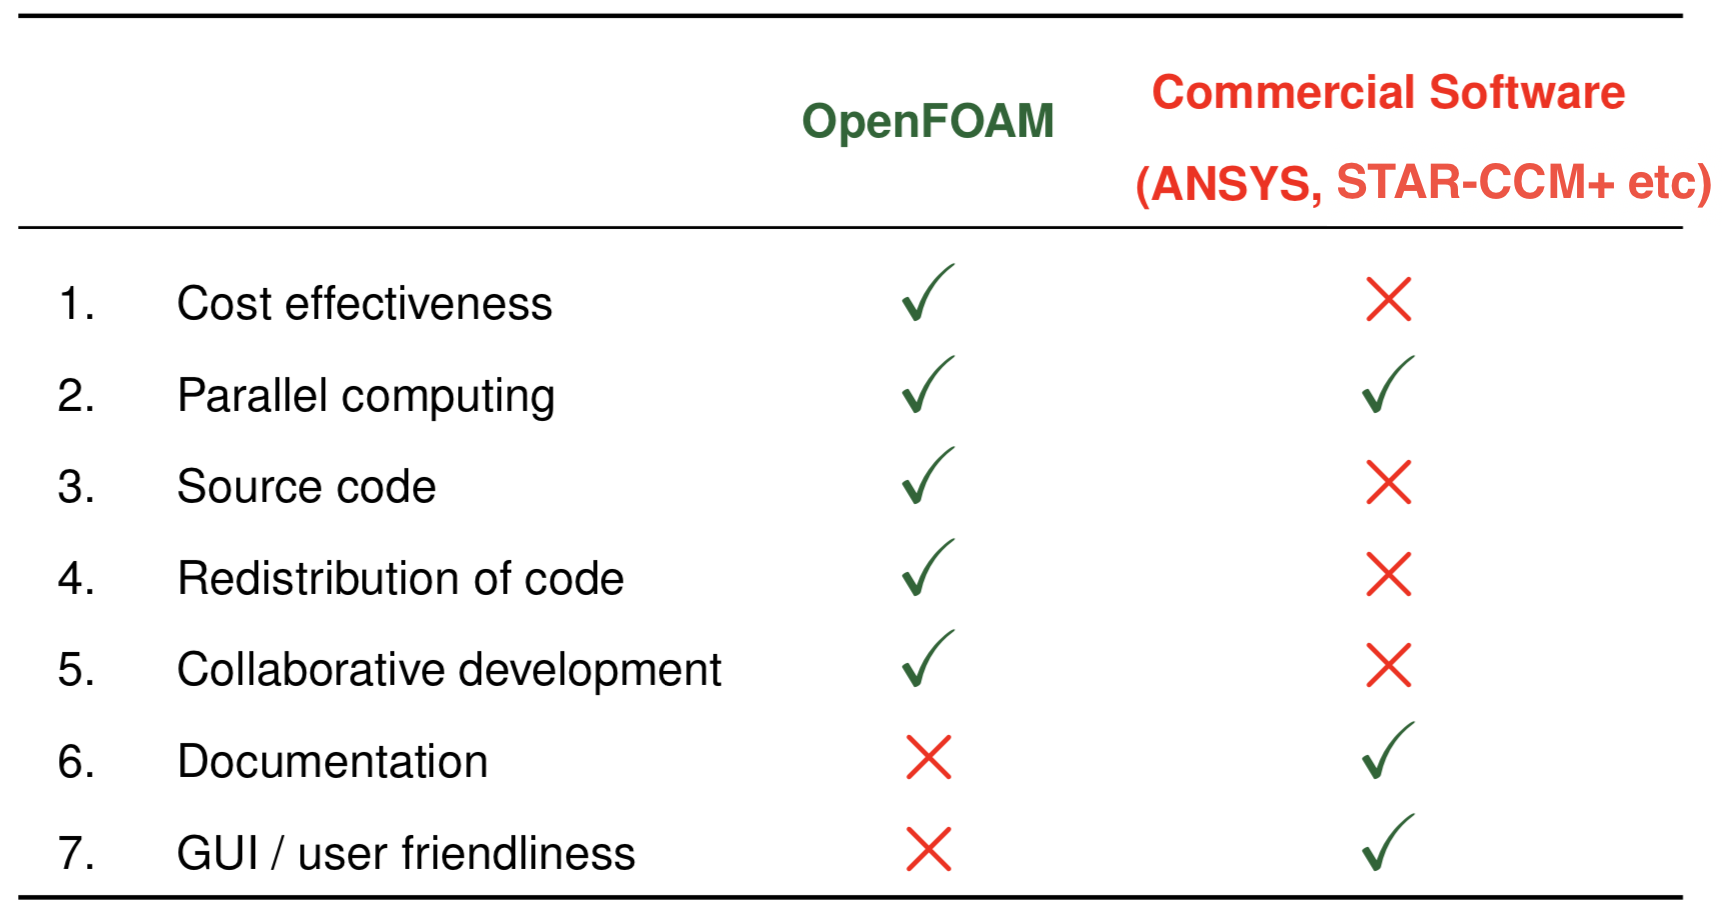
\includegraphics[trim=0cm 0cm 0cm 0cm,clip,scale=0.45]{figs/0F2.png}
\caption{ Why OpenFOAM ?}
\label{openfoam}
\end{center}
\end{figure} 
%
The simulation workflow begins with the pre-processing where the geometry along with the mesh are generated, 
%
after comes the part of choosing the solver which represent well our model, and then the post-processing where the results of the simulation are visualized.
%
The twoPhaseEulerFoam solver is the one which represents well our model and  the solver has been modified to become an isothermal flows solver, since there is no heat exchange between the phases. 
%
Then, in the constant file the different forces which act on the flow have been defined according to the assumptions made, where thus the interphase momentum exchange models have been defined.
%
Then the components of the KTGF are implemented taking into consideration the restitution coefficients. 
%
The implementation of the model also requires special attention to the boundary conditions which need a good understanding of the physical phenomenon to define them.
% %%%%
\chapter{Results and discussions} \label{results}
%
\section{Single phase flow} \label{single flow}
%
To carry out validation of the mathematical model along with the turbulence model and the treatment process for the area near the wall, simulations for a single phase flow are performed for three pipe setups. 
%
Moreover, these simulations will help to validate the approach of constructing surrogates models. 
%
The predicted values of the theoretical correlations presented in section \ref{single}, are used to judge the CFD results. 
%
The implementation of the models is done under the OpenFOAM software V7. Table \ref{table 2} summarizes different boundary conditions for different inputs. 
%
\begin{table}[ht!]
\begin{center}
\caption{Summary of the selected boundary conditions}
\begin{tabular}{cccc}
\hline Field & Inlet & Outlet & Solid walls  \\
\hline
\(\epsilon_{W}\) & fixedValue & zeroGradient & wall function\\
\(k_{W}\) & fixedValue & zeroGradient & wall function \\
\(v_{t}\) & zeroGradient & zeroGradient & wallFunction \\
\(p\) & zeroGradient & atmospheric pressure & zeroGradient  \\
\(U_W\) & fixedValue  & zeroGradient & noSlip \\
\hline
\label{table 2}
\end{tabular}
\end{center}
\end{table}

% %%%%%%%%%%%%%%%%%%%
\subsubsection{Horizontal pipe}
%
The geometry consists of a 40 $m$ horizontal pipe, with an internal diameter of 0.9 $m$. 
%
Figure \ref{horiz}(a) and \ref{horiz}(b), shows a 2D section and the 3D meshed geometry. 
%
GMSH software was used to generate a specific mesh which takes into account the near-wall refinement by calculating the height of the first cell on the wall, with a precise magnification ratio which is linked to $y^{+}$ while approaching the center of the pipe. 
%
The flow consists of water with a density $\rho=1000 kg/m^3$. 
%
The Wall roughness is set at 0.045 $mm$. The inlet velocity is in ranges of 1 to 3 $m/s$. 
%
The pressure at the outlet is fixed as atmospheric pressure. The latter initial condition is the same for the next simulations of inclined and bended pipe in subsections \ref{inclined} and \ref{bended} respectively.
%
\begin{figure}[ht!]
\centering
\begin{subfigure}{0.40\textwidth}\centering 
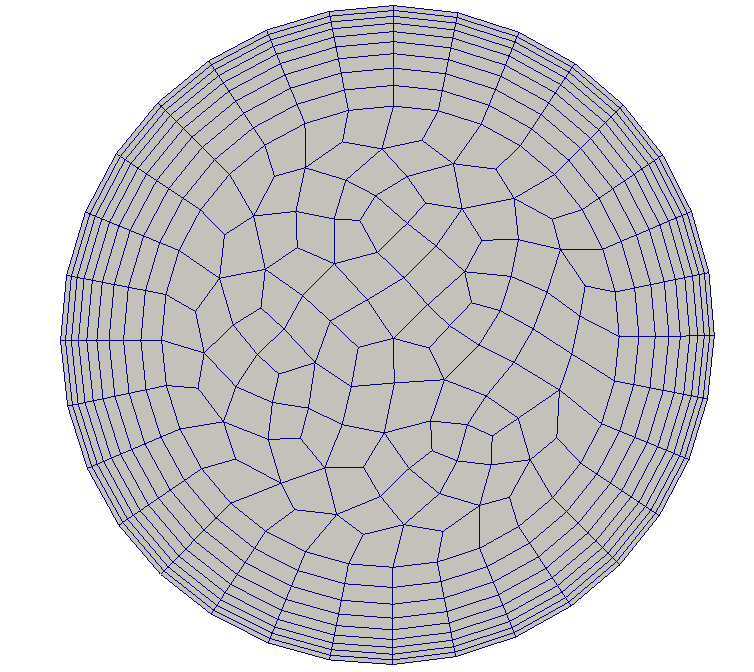
\includegraphics[scale=0.09]{figs/section.png}
\caption{}
\end{subfigure}
% 
\begin{subfigure}{0.40\textwidth}\centering 
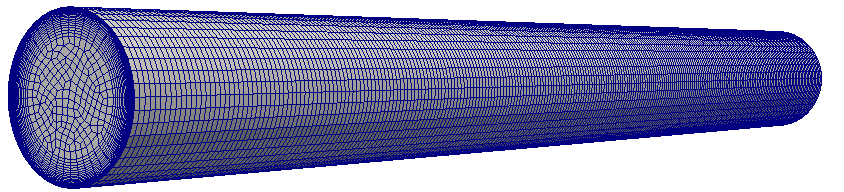
\includegraphics[scale = 0.25]{figs/HP-2.png}
\caption{}
\end{subfigure}
% %  
\caption{Horizontal pipe geometry: (a) Cross-section mesh, (b) Profile mesh }
\label{horiz}
\end{figure}

For a horizontal pipe, we have regular pressure drops, which are generated by the friction of the fluid on the internal wall of the pipe throughout its passage. 
%
They depend on, the length of the pipe, the relative roughness of the pipe, the speed of the fluid circulating in the pipe ($U_{in}$ $m/s$), as presented in table 1. 
%
Therefore, As can be seen in Figure \ref{horiz:theo}, the pressure losses are increasing relatively with inlet velocities. 
%
For this current case of a horizontal pipe, experimental data were found for water flow in (\citet{Randal-2004}), and also a good agreement was found with cfd results as shown in Figure \ref{horiz:theo}.\\
%
The mean average percentage error is defined as follows:
%
\footnotesize{$$
\text{MAPE}=\left\{\frac{1}{n} \sum_{k=1}^{n}\left[\frac{(d p / d x)_{\text{pred}}-(d p / d x)_{\text{theory} }}{(d p / d x)_{\text{theory}}}\right]\right\} 100
$$\\
\text{MAPE} = 1.21 $\%$}
\begin{figure}[ht!]
\begin{center}
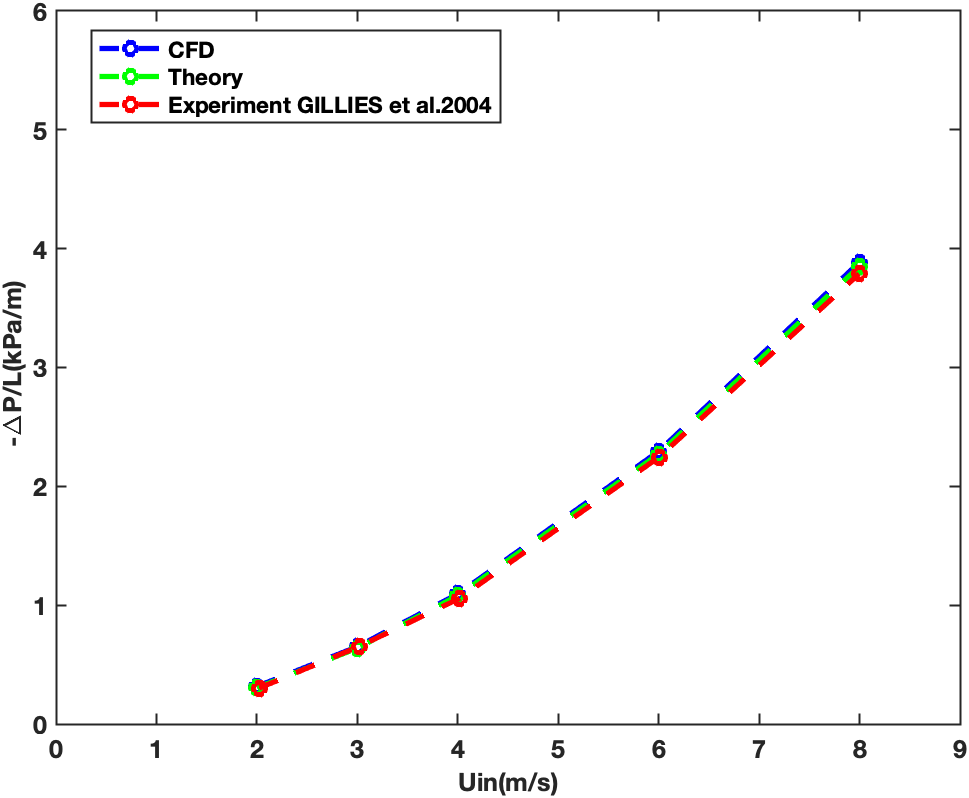
\includegraphics[scale = 0.45]{figs/WH}
\caption{ Pressure drop in horizontal pipe. 
%
Present pressure drops from CFD simulations versus empirical formula in table \ref{tab:PD} and experimental measurements.}\label{horiz:theo}
%
\end{center}
\end{figure}



 \subsubsection{Inclined pipe}\label{inclined}
 %
 In this section, the geometry consists of a 40 $m$ inclined pipe with 0.9 $m$ diameter and a 5.73 degree negative slope. Figure \ref{incline}(a) and \ref{incline}(b) show the
 cross-section and profile mesh.\\
%
\begin{figure}[ht!]
\centering
\begin{subfigure}{0.40\textwidth}
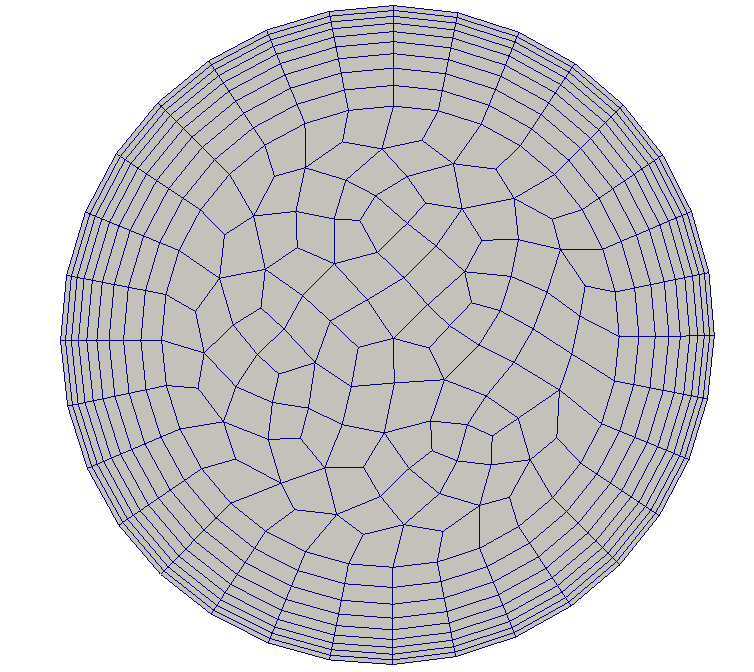
\includegraphics[scale =0.09]{figs/section.png}
\caption{}
\end{subfigure}
\begin{subfigure}{0.40\textwidth}
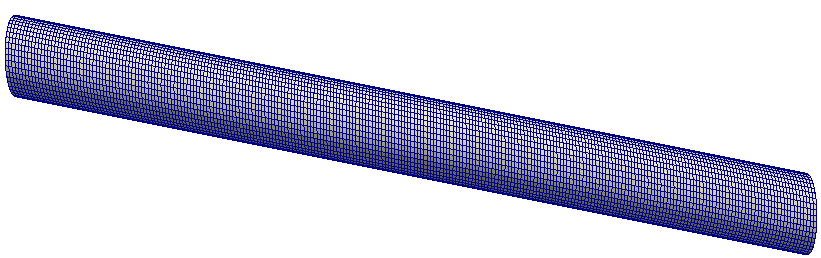
\includegraphics[width=6cm,height=2.5cm]{figs/IP}
\end{subfigure}
\caption{Inclined pipe geometry: (a) Cross-section mesh, (b) Profile mesh }
\label{incline}
\end{figure}

 Concerning this pipe setup, it is characterized by a changing elevation. 
 %
 Consequently, at the end of the inclined pipe there is the full weight of fluid pushing down on that point and due to this, 
 %
 the pressure at that point increases. 
 %
 Therefore, there is a pressure gain in the pipe as the fluid goes down. 
 %
 The total pressure difference can be calculated by adding the hydrostatic pressure to the friction component as in table \ref{tab:PD}.
 %
 Figure \ref{inclin}, show the pressure gradient as a function of inlet velocities.
 %
 As noticed the pressure gain decreases while increasing the velocity, and this comes back to the augmentation of  friction losses.\\
 %

 % \small{The mean average percentage error (MAPE) = 0.97 $\%$}
%
 \begin{figure}[ht!]
 \begin{center}
 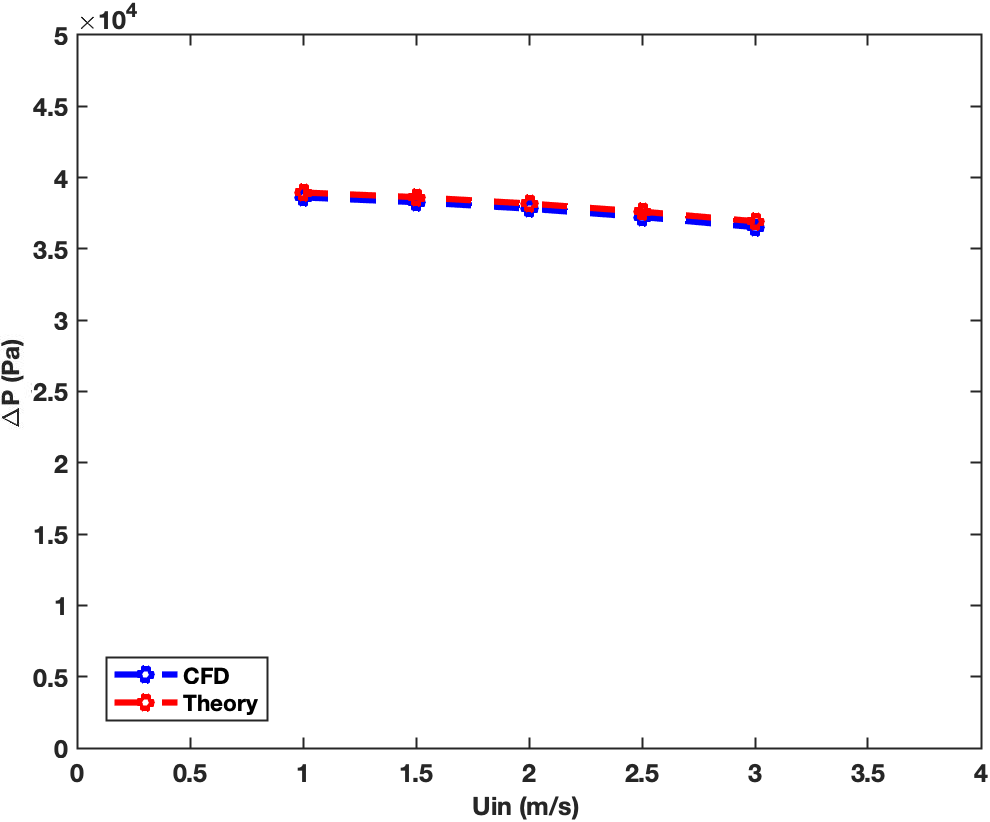
\includegraphics[scale = 0.45]{figs/inclined.png}
 \caption{ Pressure drop in inclined pipe}
 \label{inclin}
 \end{center}
 \end{figure}


%%%%%%%%%%%%%%%%%%%%%
%
 \subsubsection{Bended pipe}\label{bended}
 For this setup, the geometry consists of a $45$ degree bended pipe, of 6 $m$ equivalent length with 0.9 $m$ diameter. Figure \ref{bend}(a) and \ref{bend}(b) show the cross-section and profile mesh.

\begin{figure}[ht!]
\centering
\begin{subfigure}{0.40\textwidth}
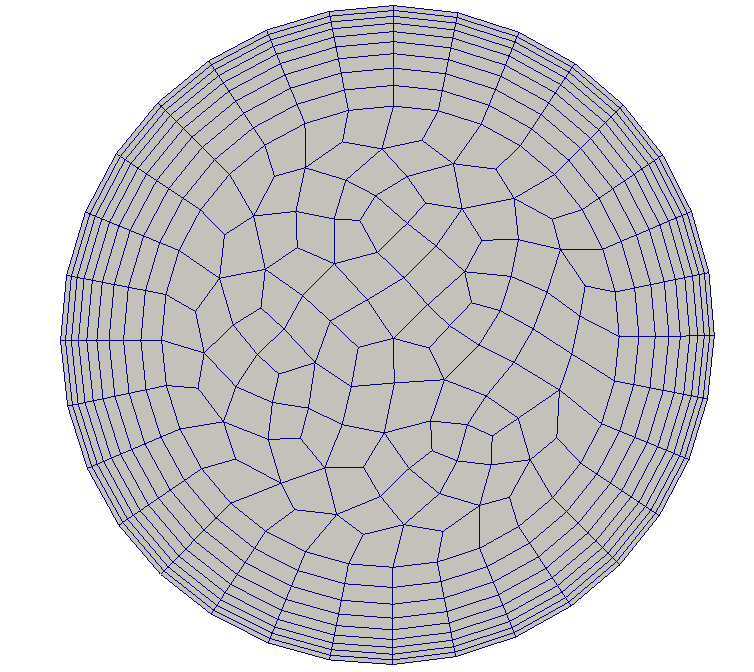
\includegraphics[scale =0.09]{figs/section.png}
\caption{}
\end{subfigure}
\begin{subfigure}{0.40\textwidth}
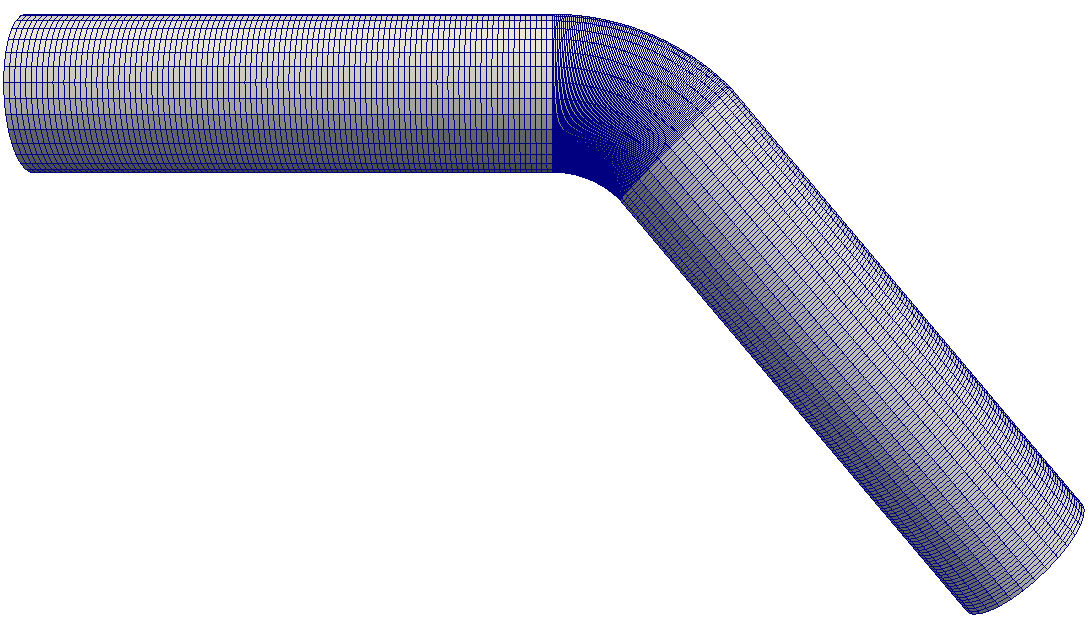
\includegraphics[scale = 0.17]{figs/bend.png}
\caption{}
\end{subfigure}
\caption{Bended pipe geometry: (a) Cross-section mesh, (b) Profile mesh }
\label{bend}
\end{figure}
%
 This pipe setup is more complex, since in addition to the previously discussed components of the  kinetic losses, another component is added namely the singular pressure drop as in table \ref{tab:PD}. 
 %
 The singular pressure drops are mainly due to the geometric modification of the pipe, such as changes of direction like bends. 
 %
 Figure \ref{bend:theo} shows that the pressure loss is increased in such geometries.

%
\begin{figure}[ht!]
 \begin{center}
 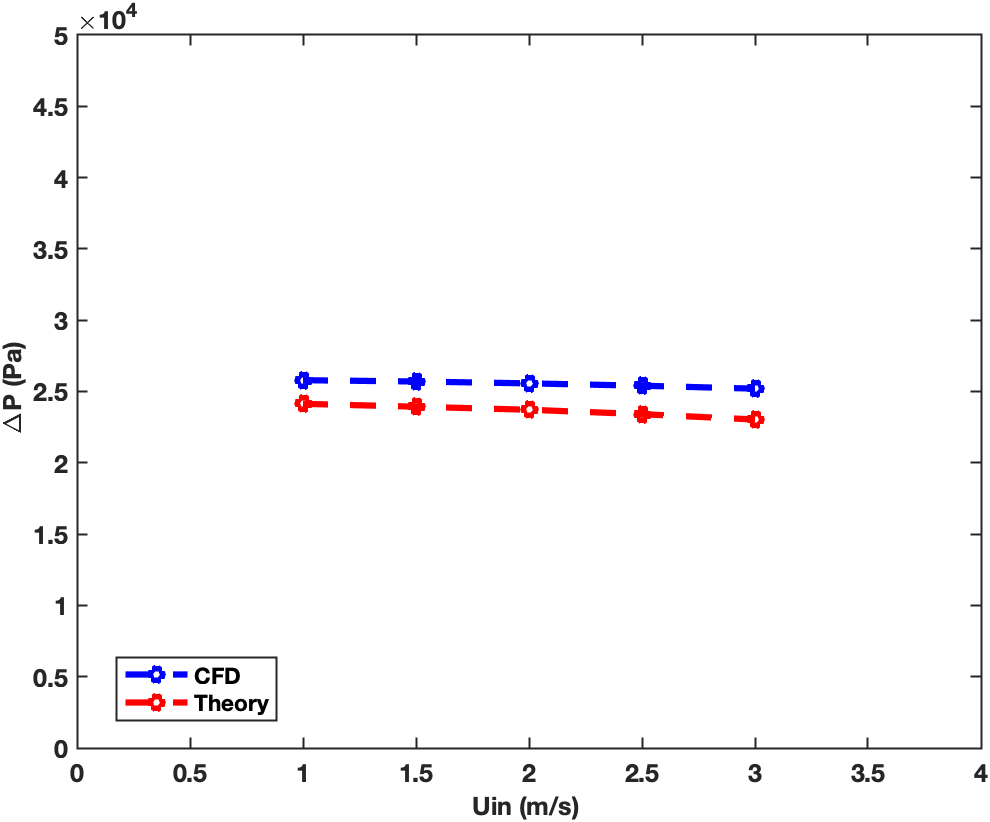
\includegraphics[scale = 0.45]{figs/bend1}
 \caption{ Pressure drop in bended pipe. The empirical formula slightly underestimates the pressure drop versus the CFD simulations }
 \label{bend:theo}
 \end{center}
 \end{figure}
 %
The pressure drop formulae constitute surrogate models for pressures calculations in piping systems with newtonian fluids such as water. 
%
From the previous analysis we see that CFD reproduces very well the pressure drop measurement and the empirical models fits the CFD results for the classical geometrical configurations. 
%
Hence, one can consider for example computing other pressure drop models for Newtonien fluids but for much more complex geometries, where experiments may be complex or time consuming to conduct. 
%
In the next section we will consider a different case, where the complexity is introduced in the fluid itself. And the aim is to use the CFD approach to develop pressure drop models for complex fluids.
%
Morevoer, once the simulations validated they can be used to develop response models (or surrogate models) for other physical quantities than pressure drops. 
%
For instance, in a slurry pipe flow a sedimentation model along pipe of different geometries can be usefull for applications.  

\section{Two phase flow} \label{Two Phase}

An attempt to simulate the behaviour of a sediment-water mixture during its transportation through a pipe has been made, using the twoPhaseEulerFoam solver available in the 6.0 release of the open-source CFD toolbox OpenFOAM. 
%
The geometry used consisted of a pipe of length L = 0.02 m, a diameter D = 0.0001 m. 
%
The flow is laminar with Re = 144,  , $\rho_S= 1,450  kg/m^3$, $\rho_W= 1,027  kg/m^3$, $V_{mixture} = 1 m/s$, $d_S= 70 \mu m$, $\mu_W = 0.00891  kg/m.s$, $\alpha_{0S} = 30 \%$, $P_0=10^5  Pa$. 
%
Figure 6 and 7, show the 2D and 3D meshed geometry. OpenFOAM's meshing utility blockMesh was used to generate structured orthogonal meshes about 200 cells along the pipe.
%
\begin{itemize}
 \bf{\item Pre-processing: 2D and 3D meshed geometry}
  \end{itemize}
 \vspace{0.5cm}
\vspace{-0.6cm}
\begin{figure}[ht!]
 \begin{center}
 \include{diag}
 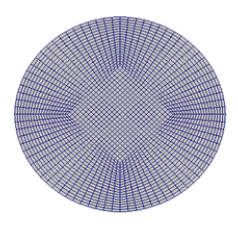
\includegraphics[trim=0cm 0cm 0cm 0cm,clip,scale=0.6]{figs/1.png}
 \caption{ Cross-section mesh}
 \label{fig:gauss}
 \end{center}
 \end{figure} 
%
 \begin{figure}[ht!]
 \begin{center}
 \include{diag}
 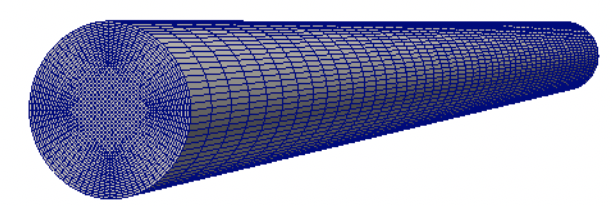
\includegraphics[trim=0cm 0cm 0cm 0cm,clip,scale=0.6]{figs/2.png}
 \caption{ 3D pipe mesh}
 \label{fig:gauss}
 \end{center}
 \end{figure} 
%
 \begin{itemize}
 \bf{\item Post-processing}
 \end{itemize}
 %
 Figure 8 and 9 show the solid concentration for the cross-section of the pipe and along the pipe respectively. 
 %
 These first results show an agreement with one of the types of two-phase flows found in the literature, which is a sliding bed flow. 
 %
 While, figure 10 shows that the condition of the fractional volumes sum for the two phases is equal to 1, throughout the diameter in the  pipe outlet.\\
 %
\begin{figure}[ht!]
 \begin{center}
 \include{diag}
 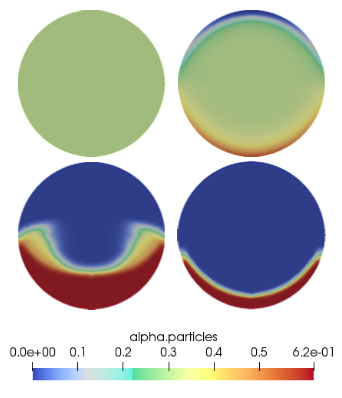
\includegraphics[trim=0cm 0cm 0cm 0cm,clip,scale=0.7]{figs/7.png}
 \caption{ \footnotesize{Cross-section Concentration at the outlet} }
 \label{fig:gauss}
 \end{center}
 \end{figure} 
%
 \begin{figure}[ht!]
 \begin{center}
\include{diag}
 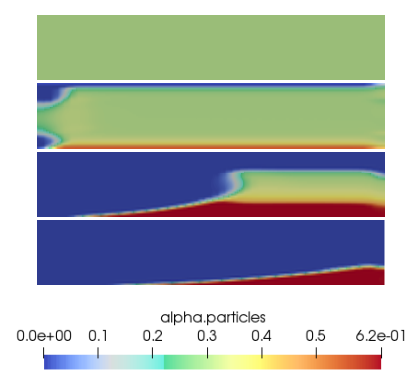
\includegraphics[trim=0cm 0cm 0cm 0cm,clip,scale=0.72]{figs/6.png}
 {\caption{ \footnotesize Concentration along the pipe}}
 \label{fig:gauss}
 \end{center}
 \end{figure} 
%
 \begin{figure}[ht!]
 \begin{center}
 \include{diag}
 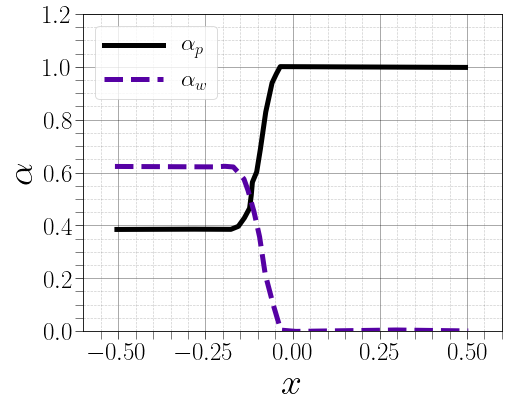
\includegraphics[trim=0cm 0cm 0cm 0cm,clip,scale=0.25]{figs/5.png}
 \caption{ \footnotesize { Volume fraction of both phases }}
 \label{fig:gauss}
 \end{center}
 \end{figure} 

 \begin{center}
 \end{center}
 Two phase simulations were presented by authors in (\citet{elkarii2020towards}), where a slurry of mono-dispersed spherical polystyrene beads with rhodorsil silicone oil were simulated in a laminar flow. 
 %
 Figure \ref{fig:laminar} shows the evolution of the solid concentration profile of the mixture over time.\\
 %
\begin{figure}[ht!]
 \begin{center}
 (a)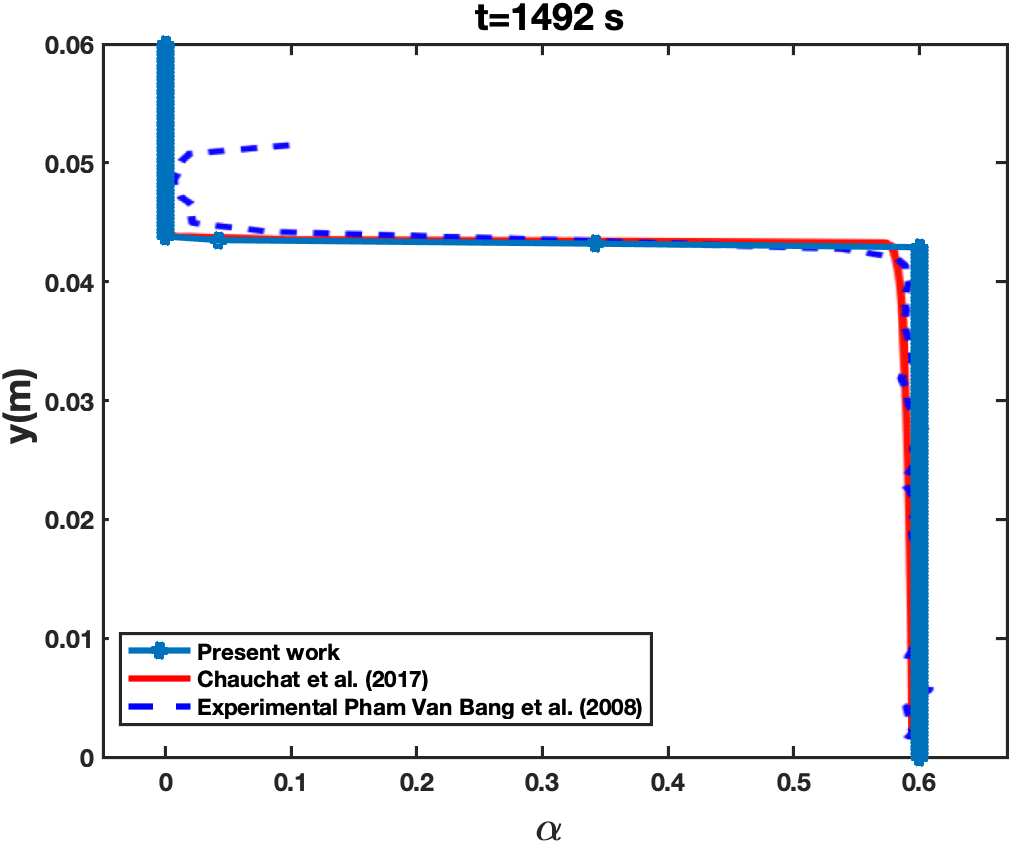
\includegraphics[scale = 0.45]{figs/E4}
 \end{center}
 \end{figure}
%
 \begin{figure}[ht!]
 \begin{center}
 (b)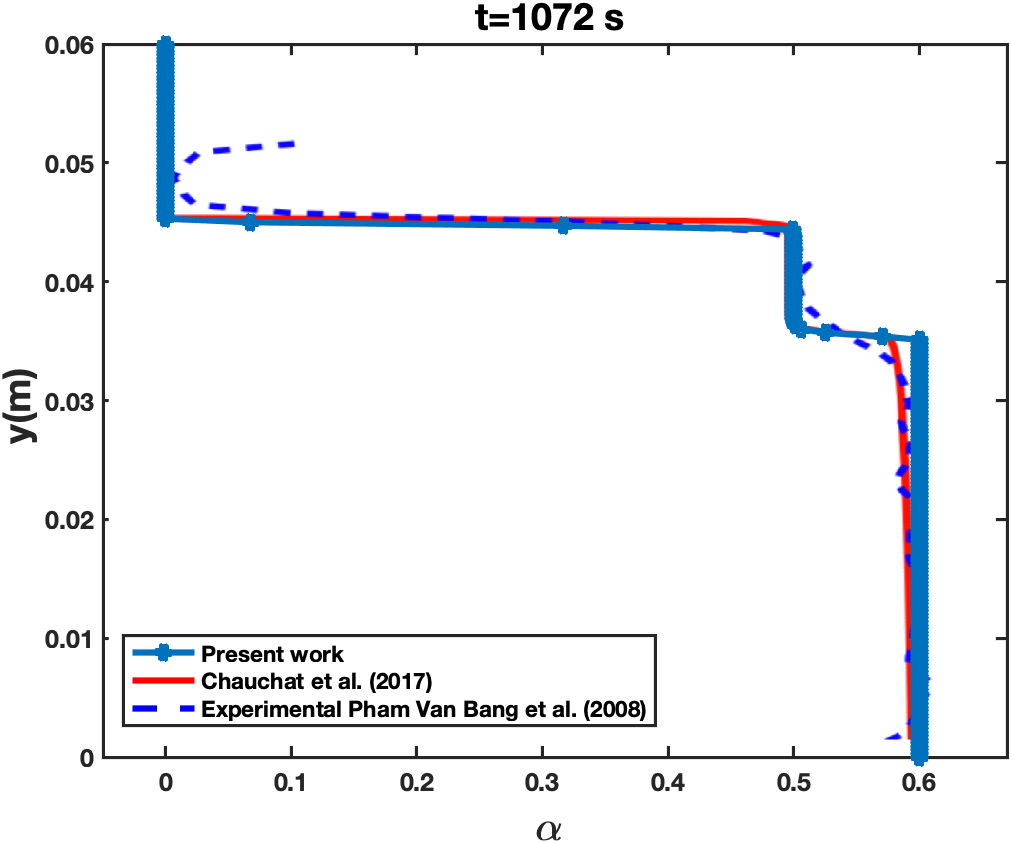
\includegraphics[scale = 0.45]{figs/E3}
 \end{center}
 \end{figure}
%
 \begin{figure}[ht!]
 \begin{center}
 (c)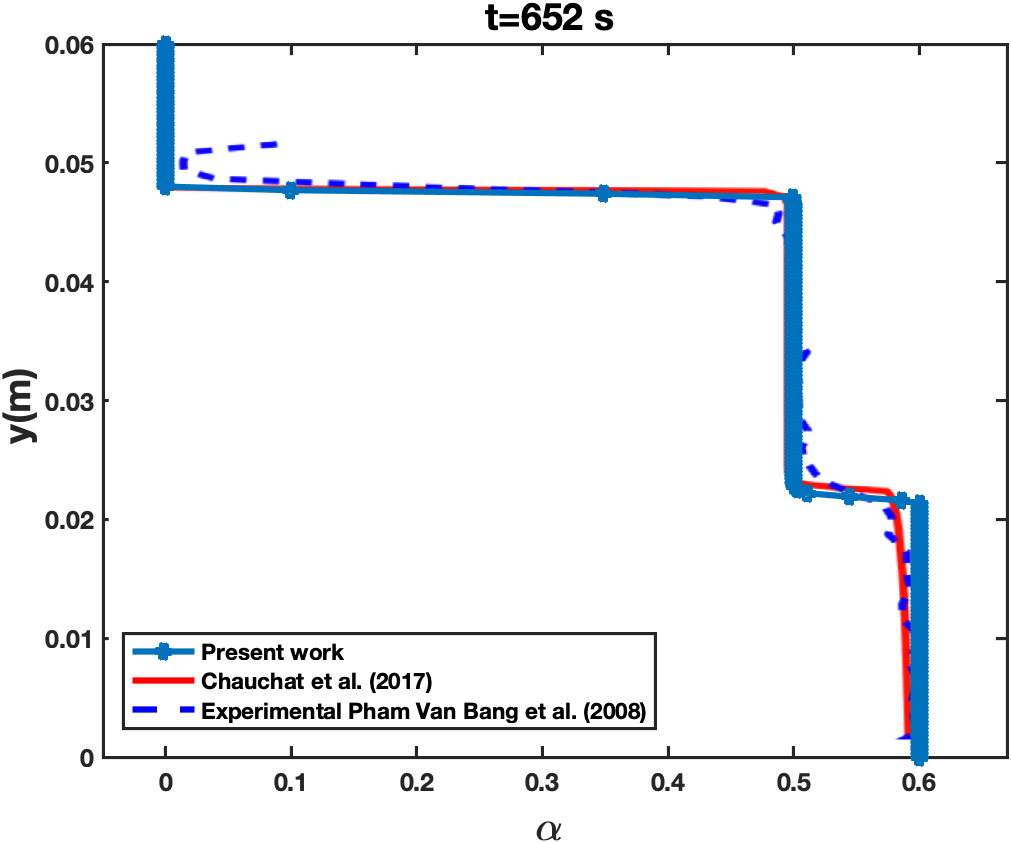
\includegraphics[scale = 0.45]{figs/E2}
 \end{center}
 \end{figure}
%
 \begin{figure}[ht!]
 \begin{center}
 (d)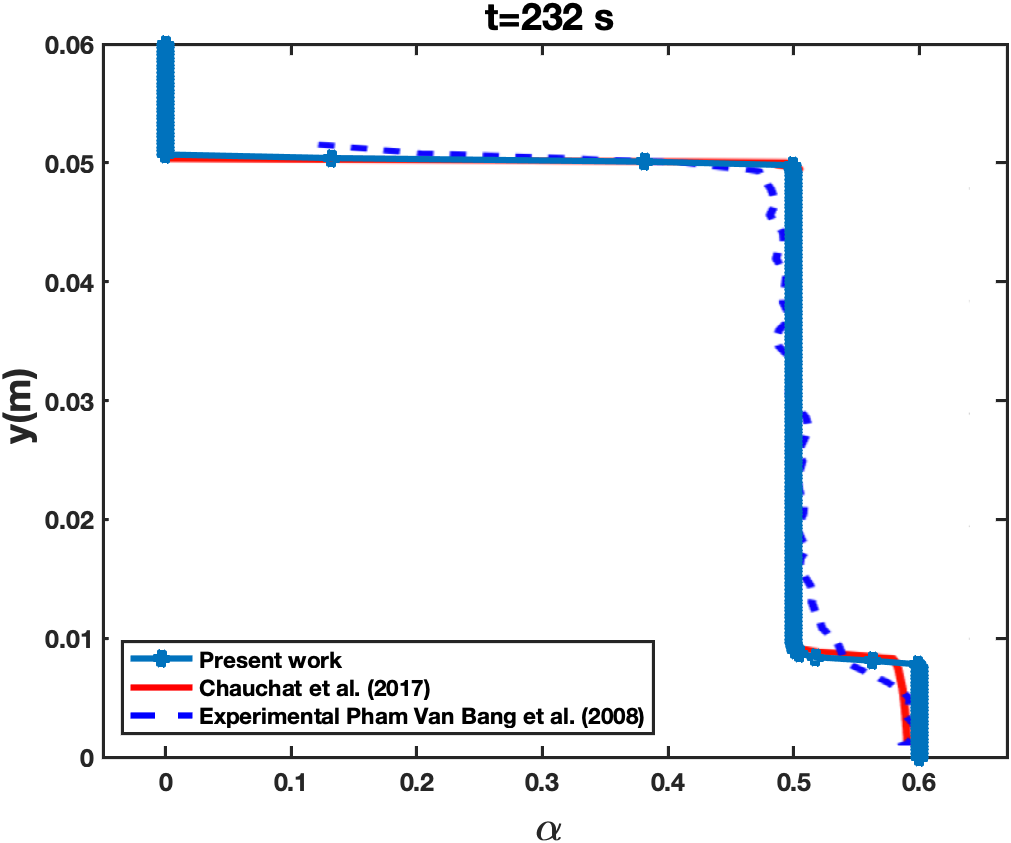
\includegraphics[scale = 0.45]{figs/E1}
 \end{center}
 \end{figure}
%
 \begin{figure}[ht!]
 \centering
 \caption{Sediment concentration profiles over time (a) At t = 232 s, (b) t = 652 s (c) t = 1072 s (d) t = 1492 s}
 \label{fig:laminar}
 \end{figure}
%
The previous study (\citet{elkarii2020towards}), validates the model for its capability to reproduce and predict high volume concentration profiles up to 60 $\%$. 
%
The validation case consists of a sedimentation of non-cohesive particles by \citet{chauchat}, based on experimental data from (\citet{Pha-2008}). 
%
The sedimentary phase was also modeled as continuous and consecutive laws were adopted to take sedimentary constraints into account.
%
 However, to approach the simulation of a real slurry flow, the turbulence aspect must be added to prevent sedimentation problems. 
 %
 Therefore, in this part, CFD simulations were performed to fit the experimental results of a turbulent flow of water-sand slurry under isothermal conditions, reported by \citet{Randal-2004}. 
 %
 Experimental data consists of pressure drops along the pipe, particle concentration profiles and particles velocity profiles at the pipe outlet. 
 %
 The simulation domain consists of a 10 m long pipe. boundary conditions set are the inlet, the outlet and the lateral surface which is referenced as walls, are presented in the table \ref{tab:bc}. 
 %
 The mass flow rates of the two phases, \(\dot{m}_{W}\) and \(\dot{m}_{\mathrm{S}}\) are fixed at the inlet boundary, and calculated as in Eq.(\ref{mass rate}), the turbulent kinetic energy of the liquid, \(k_{in}\), 
 %
 and its dissipation rate, \(\epsilon_{in }\), were also fixed as in Eq.(\ref{kin}) and Eq.(\ref{epsilon in}). 
 %
\begin{equation}
 \dot{m}_{W}= \alpha_{\mathrm{W}} \rho_{W} U_{\mathrm{W}} A;\quad \dot{m}_{\mathrm{S}}= \alpha_{\mathrm{S}} \rho_{\mathrm{S}} U_{\mathrm{S}} A
 \label{mass rate}
 \end{equation}
%
 \begin{table}[ht!]
 \begin{center}
 \caption{Summary of the selected boundary conditions}
 \label{tab:bc}
 \begin{tabular}{cccc}
 \hline Field & Inlet & Outlet & Solid walls  \\
 \hline\(\alpha_{s}\) & fixedValue & zeroGradient & zeroGradient \\
 \(\alpha_{W}\) & fixedValue & zeroGradient & zeroGradient \\
 \(\epsilon_{W}\) & fixedValue & zeroGradient & wall function\\
 \(k_{W}\) & fixedValue & zeroGradient & wall function \\
 \(v_{t}\) & zeroGradient & zeroGradient &  wall function \\
 \(p\) & fixedFluxPressure & atmospheric pressure & zeroGradient \\
 \(\theta_{p}\) & fixedValue & zeroGradient & JohnsonJacksonParticleTheta\\
 \(U_{W}\) & mass flow rate  & zeroGradient & noSlip\\
 \(U_{S}\) & mass flow rate  & zeroGradient & JohnsonJacksonParticleSlip  \\
 \hline
 \end{tabular}
 \end{center}
 \end{table}
%
The numerical simulations performed in this section, uses the same mesh configuration, as in section \ref{single flow}, except that the meshes have been refined in all directions. 
%
The flow is characterized by high inlet velocities ranging up to 8 $m/s$. 
%
Two diameters of particles are considered, along with different solid concentrations. 
%
The physical parameters used are sand density $\rho_s=2650$ $kg/m^3$, water density $\rho_W=1000$ $kg/m^3$, and water viscosity $\mu_w= 10^{-3} kg/m.s$. 
%
The radial distributions of sand particles for two inlet concentrations are presented in figure \ref{solid}. 
%
Regarding the experimental results, the solid concentration profile varies slightly along the diameter of the pipe ($ 0.19 <\alpha_s <$ 0.24). 
%
The present simulation in figure \ref{solid}(a) agrees fairly well with the experiments in the bulk flow $(0.2<r/D <0.9)$, whereas the model underestimate the experimental values of $ \alpha_s $ near the upper wall ($ r / D> 0.9 $), and on the other hand, 
%
overestimate them along the lower wall ($ r / D <0.2 $ ). In the present model, it can be attributed to the none total control of the turbulent viscosity term, which promotes the phenomenon of sedimentation, resulting in a non-homogeneous concentration profile. 
%
On figure \ref{solid}(b) the solid concentration is increased up to $33$ $\%$, but, the same behavior is always observed, and corresponds to a pseudo-homogeneous flow with formation of a small bed of particles.  \\
%
\begin{figure}[ht!]
 \begin{center}
 (a)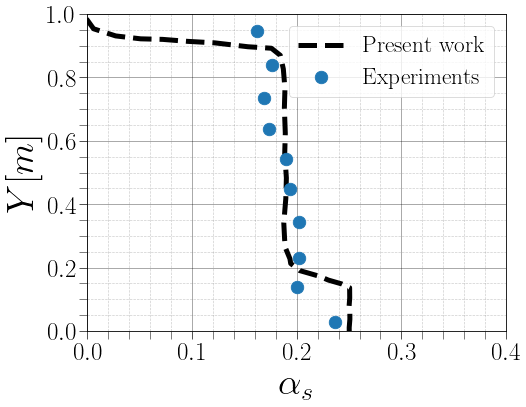
\includegraphics[scale = 0.3]{figs/3C}
 \end{center}
 \end{figure}
%
 \begin{figure}[ht!]
 \begin{center}
 (b)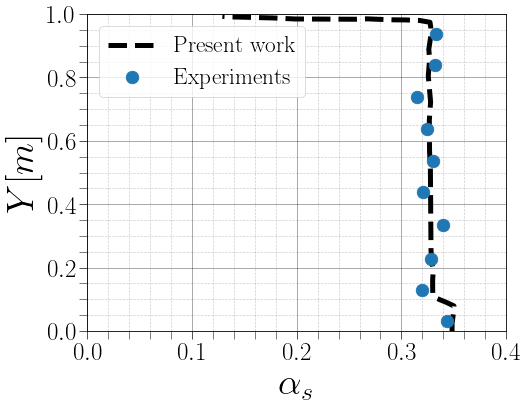
\includegraphics[scale = 0.3]{figs/C33}
 \end{center}
 \end{figure}
%
 \begin{figure}[ht!]
 \centering
 \caption{Radial distributions of the volume fraction of sand particles of $d_p= 0.09 mm$ for $U_{in} = 3 m/s$: (a) ($\alpha_{s,in}$ = 0.19), (b) ($\alpha_{s,in}$ = 0.33) }
 \label{solid}
 \end{figure}
 %
 The particles velocity  profiles for $U_{in} = 2 m/s$ and $U_{in} = 3 m/s$ are presented in figure \ref{U}(a) and \ref{U}(b) respectively. 
 %
 On the contrary to the concentration distribution, the present model predicts the right profile of velocity. 
 %
 It is remarked that the axial average velocities  distributions are symmetrical, and they agree almost exactly to a classic turbulent parabolic profile. 
 %
 This comes down to the fact that the presence of particles does not greatly influence the current field. 
 %
 This is explained by the constant solid concentration around the value 0.2 for the entire pipe and the dynamic viscosity of the fluid then varies slightly.\\
%
 \begin{figure}[ht!]
 \begin{center}
 (a)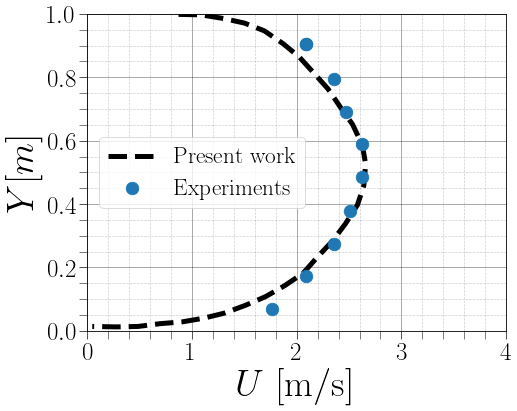
\includegraphics[scale = 0.3]{figs/V22}
 \end{center}
 \end{figure}
%
 \begin{figure}[ht!]
 \begin{center}
 (b)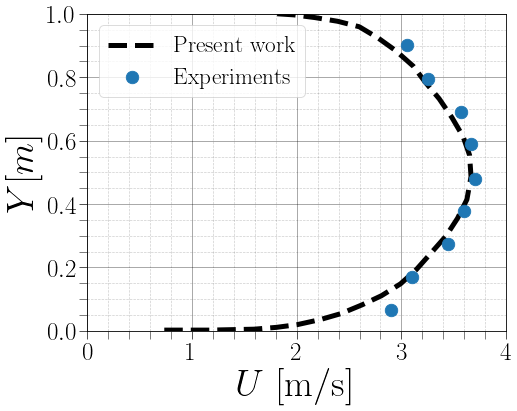
\includegraphics[scale = 0.3]{figs/3CFD}
 \end{center}
 \end{figure}
%
\begin{figure}[ht!]
 \centering
 \caption{Radial distributions of the mean axial velocity of sand particles at the outlet of the pipe, for $\alpha_{s}in$ = 0.19 and $d_p= 0.09 mm$ : (a) ( $Uin = 2 m/s$), (b) ( $Uin = 3 m/s$).}\label{U}
 \end{figure}
%
 Figure \ref{P} (a) and (b) shows the variations of the pressure drop per unit length $ \Delta P/L $ with the inlet velocity of the mixture $ U_{in}$. 
 %
 The present simulations obtained for two different particles diameters $d = 0.09 mm$ and $d=0.27 mm$, for nearly the same inlet concentration, and for a high velocities. 
 %
 Experimental data from (\citet {Randal-2004}) is used as a validation for current simulations. 
 %
 The pressure drop analyzed in current simulations augments almost linearly with $ U_{in} $. 
 %
 As anticipated, the pressure drop increases  because of the increased values of friction losses. 
 %
 Results fit well in figure \ref{P} (a) for $d=0.09 mm$, However, discrepancies are higher at high velocities. 
 %
 Contrary to figure \ref{P} (b) for $d= 0.27 mm$, a very good agreement is observed at high velocities, and a large gap is visible at low input velocities $U_{in} \leq 3 m/s$.\\
%
 \begin{figure}[ht!]
 \begin{center}
 (a)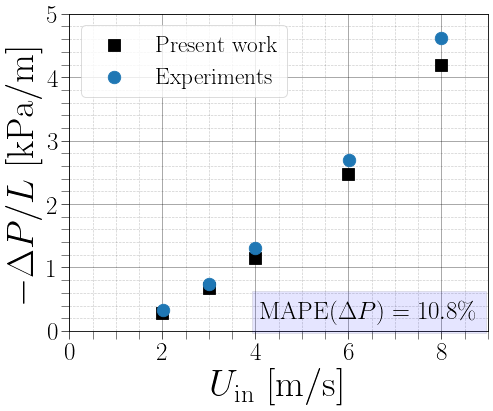
\includegraphics[scale = 0.3]{figs/DP009}
 \end{center}
 \end{figure}
%
 \begin{figure}[ht!]
 \begin{center}
 (b)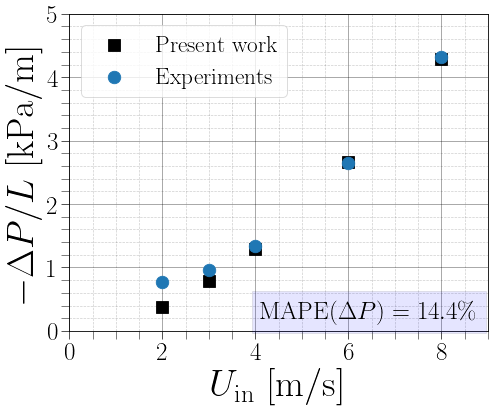
\includegraphics[scale = 0.3]{figs/DP27}
 \end{center}
 \end{figure}
 %
\begin{figure}[ht!]
 \centering
 \caption{Pressure drop per unit of length $\Delta P/L$  versus slurry velocity: (a) ($\alpha_S=0.19$, $d=0.09 mm$), (b) ($\alpha_S=0.20$, $d=0.27 mm$).}
 \label{P}
 \end{figure}
 %
 It is also noted, that coarser particles compared to smaller ones, have superior pressure drop at lower flow rates and have an inferior one at higher flow rates.  
 %
 The reason behind this, is that the coarser particles at lower speeds deposit more which comes down to the gravitational effect, and subsequently, the amount of particles in the bed increases which leads to more frictions. 
 %
 While, in the case of smaller particles at higher velocities, the  pressure losses are bigger due to the larger surface area of the material.
 %
% %%%%%%%%%%
\section{Surrogate model}
%
 Once the CFD results are validated with experimental data, this work aims to construct a surrogate model for the pressure drops for a two-phase flow within a piping system. 
 %
 The proposed model uses the empirical formula in Table \ref{tab:PD} for the pressure losses due to frictions for horizontal pipes. 
 %
 The density, however, is that of the water-sand mixture. 
 %
 The model has been calibrated to find the optimal friction factor f, that fit well with the CFD results trough a minimization process (figure \ref{optimal}), for different solid concentration $\alpha_s$ and two particle sizes $d_p$. 
 %
 So that the calculations of the pressure drops by the empirical formula correspond well to the CFD results. 
%
 \begin{figure}[ht!]
 \begin{center}
 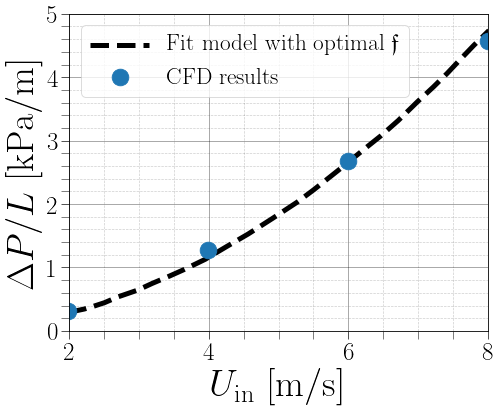
\includegraphics[scale = 0.35]{figs/alpha3D0.png}
 \caption{Example of fitting of the empirical formula of pressure drop with the CFD results for $\alpha_S = 0.19$ and $d_p = 0.09 mm$.}
 \label{optimal}
 \end{center}
 \end{figure}
%
 Figure \ref{surro} shows the variation of the calibrated friction factor $f(\alpha_s,d_p)$ as function of the solid volume concentration for two different particle sizes.
 \begin{figure}[ht!]
 \begin{center}
 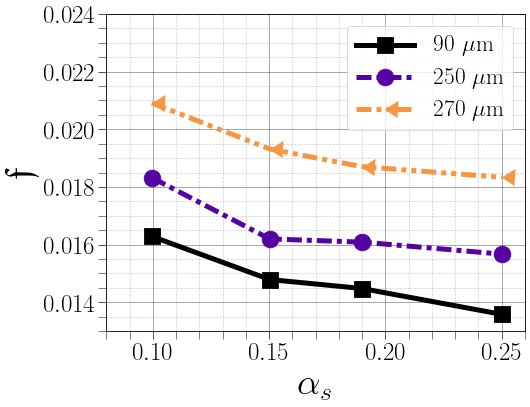
\includegraphics[scale = 0.35]{figs/suur.png}
 \caption{Optimal calibrated values of the friction factor along with the variation of the solid concentration for particles with diameter $d_p=0.09$ and $d_p=0.27$.}
 \label{surro}
 \end{center}
 \end{figure}
 According to figure \ref{surro}, one can for example for a given $\alpha_S$ and the specified particle diameters, interpolate to find values of f and then predict the pressure drop by substituting the found value of f in the empirical formula.
%%%%%%%%%%%%
 \subsubsection{Generalized Polynomial Chaos (GPC)}

TBD


% %%%%%%%%%%
\chapter{Conclusion} 
%
This paper is about modelling slurry flows in pipelines. 
%
A quite vast review of the literature of previous CFD investigations on slurry flow in horizontal pipelines was realized first, to decide on the relevant modeling approaches as well as the corresponding mathematical models. 
%
Based on this state of art, the two fluid model was the one chosen to work with, because it has the ability to capture well the physics of such complex flows while ensuring moderate computing time. 
%
Then, it was decided to begin with simulations of single phase flow into different pipe setups, to validate the turbulence model and to validate the approach of constructing a surrogate model throughout 3D numerical simulations. 
%
In this part CFD results matches the empirical data and theoretical models for pressure loss, also a really good agreement versus experimental data even at high velocities was found. 
%
After that, two phase flow simulations are performed, to investigate the physical phenomenons within such flows.
%
 CFD results showed high level correspondence with the presented  experimental data. 
 %
 Starting with the results of the pressure drops, the overall mean relative errors are limited to 15 $ \% $, and this validates our use of the CFD experiments to build a pressure loss surrogate model. 
 %
 However, some deviation is noted for the development of the solid concentration profile along the diameter of the pipe. 
 %
 Roughly speaking, the validity of the mathematical model under the given range conditions is proven, and these results will allow us to construct pressure loss laws. 
 %
Finally, a surrogate model is tested, which makes it possible to predict the pressure drops as a function of the variation in the solid concentration without performing simulations. 
%
Further tests are to come where greater variation in parameters such as solids concentration, particle size and even pipe diameter will be taken into account to increase result's accuracy. 
%
This type of surrogate models can be incorporated for plant's operators to predict pressure drops as a function of the variation of different flow parameters.
%
However, Further simulations are now required to account for enough wide range conditions to cover different types of applications in several industries, including phosphate slurries.
%

\section*{Acknowledgement} This work was supported by "Office Chérifien des Phosphates" (OCP Group) Morocco.





\bibliography{report}



\end{document}
